%卒業論文用テンプレート
\documentstyle[graphicx]{jronbun}

%諸定義
\newenvironment{indention}[1]{\par
\addtolength{\leftskip}{#1}
\begingroup}{\endgroup\par}

%論文名
\title{\underline{IEEE802.15.4準拠の低消費電力無線通信モジュールを用いた} \\ \underline{室内環境値計測デバイスの実装}}
%教官名
\kyoukan{高橋寛教授}
\second{王森レイ講師}
%名前
\author{稲田 一輝}
%提出日
\date{令和3年2月12日提出}
%講座名
\kouza{\gt 愛媛大学工学部情報工学科情報システム工学講座}

\begin{document}
%タイトル生成
\maketitle
%目次生成
\pagenumbering{roman}
\tableofcontents
\cleardoublepage
\pagenumbering{arabic}

%--ここから本文--
%第1章 まえがき
\chapter{まえがき}
%まえがき
%1-1要約:第一文-論文の趣旨,後1~2文①考えたこと②やったこと③結果の概要④成果の意義
%1-2問題設定(序論):研究をなぜ実施しなければならないのかを書く
%①あなたが解こうとする問題は何ですか?②その問題には必要性や需要はありますか?③あなたの取り組む問題は未解明で新規のものですか?④有用性はどれくらい見込めますか?
%1-3関連研究を引用.1)定石とすべき先行研究 2)定石化されていない部分の分岐状況
%各質問に対する回答パターンについては本参照




近年,新型コロナウイルスなどの感染症の拡大が世界中で話題となっており,多くの場所に影響を及ぼしている.
例えば,あるアンケートによると全体の81.1\%の人が健康に関する意識が変化したと回答している\cite{ishiki}.
特に感染症に感染するリスクを気にする人も多く,リスクに関しての情報を正しく得るということが求められる.
新型コロナウイルスを例にとってみると,飛沫感染,および接触感染によって感染すると言われている.
特に,密閉,密集,密接といった,いわゆる「3密」によって感染リスクが高くなると言われている\cite{koronaQA}.

情報が知れ渡るとともに,次はそのような状況を作らないことが同時に求められるようになっており,各方面から呼びかけが行われている.
それらの状況を作り出さないための方法として,例えば換気が挙げられるが,実際に換気によってどの程度空気環境が変わったのかは目で見てわかるものではない.
換気によって変わった空気環境を測るための基準としては浮遊粉塵の量,一酸化炭素濃度,二酸化炭素濃度,温度,湿度などが挙げられている\cite{kanki}が,これらすべてを計測し,判断することは容易なことではない.
この中でも温度,湿度については安価に計測機器を手に入れることができるが,それだけでは感染リスクという面から見た空気状況の判断が十分に行えるとは言い難い.
一方で,愛媛大学工学部社会基盤iセンシングセンターの実験によれば,部屋の換気状況の指標として二酸化炭素濃度の計測が有用であると思われるとの結果が出ており,この計測が重要となる.

しかしながら,二酸化炭素濃度も計測できる機器においてはコンセントから常時電源供給が必要であるものがほとんどとなっている.
これではコンセントなどの電源が供給するものが近くに必要となるなど,設置場所が限られてしまう.
また,それによって複数箇所に設置するのが難しくなるため,部屋の一か所の状況しか知ることができない場合が多い.
それでは,部屋全体の状況ではなく設置する場所の特性を反映したものになってしまい,正確なデータが収集しにくいという面を持つ.
このように,設置場所が限られてしまうなどにより,理想的な場所や複数箇所に設置できないため,安易に導入できないという大きな障害が生じている.

そこで,感染リスクを環境値だけでなく,その値の総合的な良し悪しを示すことができ,かつセンサの設置場所の制限が従来のものより少ないものを作成することが必要であると考えた.
これにより,感染症への意識の高まりからくる需要を満たすことができ,それとともに感染症が広がりにくい状況を構築する一助となることが期待できる.

そこで,本研究では,部屋の中の環境を総合的な観点からモニタリングし,その感染症リスクを分かりやすく表示でき,かつそれが容易に設置できる感染症予防サポートシステムの作成を目的とした.
この目的を達成するために,本研究では,乾電池で動作し,かつ無線でセンサのデータを送信する,従来より設置場所の制約の少ない小型の室内環境値計測デバイスを開発することを目標とする.

感染症予防サポートシステム全体の開発においては,システムの設計をより洗練されたものとし,かつ短期間で行うことができるよう,グループ(伊藤大輝,稲田一輝,小田恵吏奈,掛水誠矢)で開発を行った.
開発工程においてはグループ内での分担,および設計に対する検証を容易に行うためにV字開発モデルに従って行った.
また,要求分析,基本設計,詳細設計においてはグループ内での共通認識を図るためUML(Unified Modeling Language)を使用した.

本論文の構成は下記のとおりである.
%ここから下は後で修正%
第2章では本研究で用いる用語や研究方針,本システム全体の概要について述べる.
第3章ではV字開発モデルに従った本システムの設計について述べる.
第4章では,感染症予防サポートシステムとしての環境値取集デバイスの実装と検証結果について述べる.
第5章では実装・検証した本システムの評価を行い,考察を示す.
第6章では本研究のまとめを述べる.

%ここから去年
%しかしながら,売り場規模別のセルフレジの設置率については,大規模店舗中心型が25\%を越えているのに対し,小規模や中規模の企業はそれぞれ7.1\%,7.4\%\cite{super}と低い状態となっている.
%また,今後のセルフレジの設置意向について,全国スーパーマーケット協会によるアンケートに,セルフレジを新たに設置したいと回答した割合が,都市圏では8.8\%なのに対し,地方圏では14.0\%\cite{super}と高くなっている.
%人手不足が続くなか,利用者のレジ待ち時間を解消するため,精算スピードが速くなるセルフ精算レジの導入意向が高くなっていることが分かる\cite{super}.
%人手不足の著しい地方圏のスーパーマーケットや小規模や中規模の企業へセルフレジの導入が進んでいない理由としては,コストがかかることが要因として挙げられる.
%無人レジ店舗においては数十台のカメラやセンサが必要であったり,商品すべてに独自のICタグを埋め込む必要があったりなど大きなコストを要するものとなっている.
%また,既存のスーパーマーケットにおいても,セルフレジの導入は費用の点で大きな負担がかかっているのが現実の問題としてあることが考えらえる.
%
%そこで,本研究では既存の無人レジ店舗のような複雑で高価なシステムではなく,小規模や中規模の企業でも導入できる安価なスマートモビリティレジシステムの作成を本研究の目的とした.
%この目標を達成するために,本研究では,Webカメラと超音波センサ,ロードセルなどのセンサを用い,安価なモビリティショッピング端末を開発することを目標とする.
%
%具体的には,シングルボードコンピュータであるRaspberry PiとWebカメラ,各種センサを用い,商品の識別から決済に至るまでの一連の流れを行えるシステムの開発を行った.
%システムの開発では,V字モデルに従って,グループ(段原丞治,真鍋樹)でスマートモビリティレジシステムの開発を行った.要求分析,基本設計,詳細設計の際はUML(Unified Modeling Language)を用いた.
%
%本論文の構成は下記のとおりである.第2章では本研究で用いる用語や研究方針,本システム全体の概要について述べる.
%第3章ではV字モデルに従った本システムの設計について述べる.第4章では,モビリティショッピング端末の実装と検証結果について述べる.
%第5章では実装・検証した本システムの評価を行い,考察を示す.第6章では本研究のまとめを行う.

%第2章 準備
\chapter{準備}
%第2章:準備
 本章では、システム開発の進め方と、設計の工程で作成したUML図について説明する。

\subsection*{V字モデル\cite{kumikomi}}
ソフトウェアを開発する上では、適切な開発プロセスに沿って作業を進める必要がある。本研究では、開発プロセスのモデルの一つであるV字モデルを採用し、開発を進めた。このモデルを用いた場合の、各プロセスの進め方を図\ref{buiji}に示す。このモデルではテストを重視しており、図\ref{buiji}からもわかるように、左側にある分析や設計、実装のプロセスと、各テストの工程との対応が理解しやすく、検証の段階において、検証の対象とすべき範囲が把握しやすいという利点がある。例えば、要求分析に対してはシステムテストが配置され、実装に対しては単体テストが配置されている。これは、プログラム作成などの実装の正しさを単体テストによって確認し、要求分析の正しさをシステムテストで確認することを示している。そして右側のテストの各プロセスで不具合が見つかった場合には、左側の対応するプロセスに戻って修正を行うことになる。本研究でも、このような開発プロセスモデルの手順に沿い、必要に応じて、前のプロセスに立ち返りながら、運用に至るまでのプロセスを進めた。なお、本論文ではシステムテストと同じ意味を持つ言葉として、総合テストという言葉を用いている。

\begin{figure}[htbp]
	\centering
	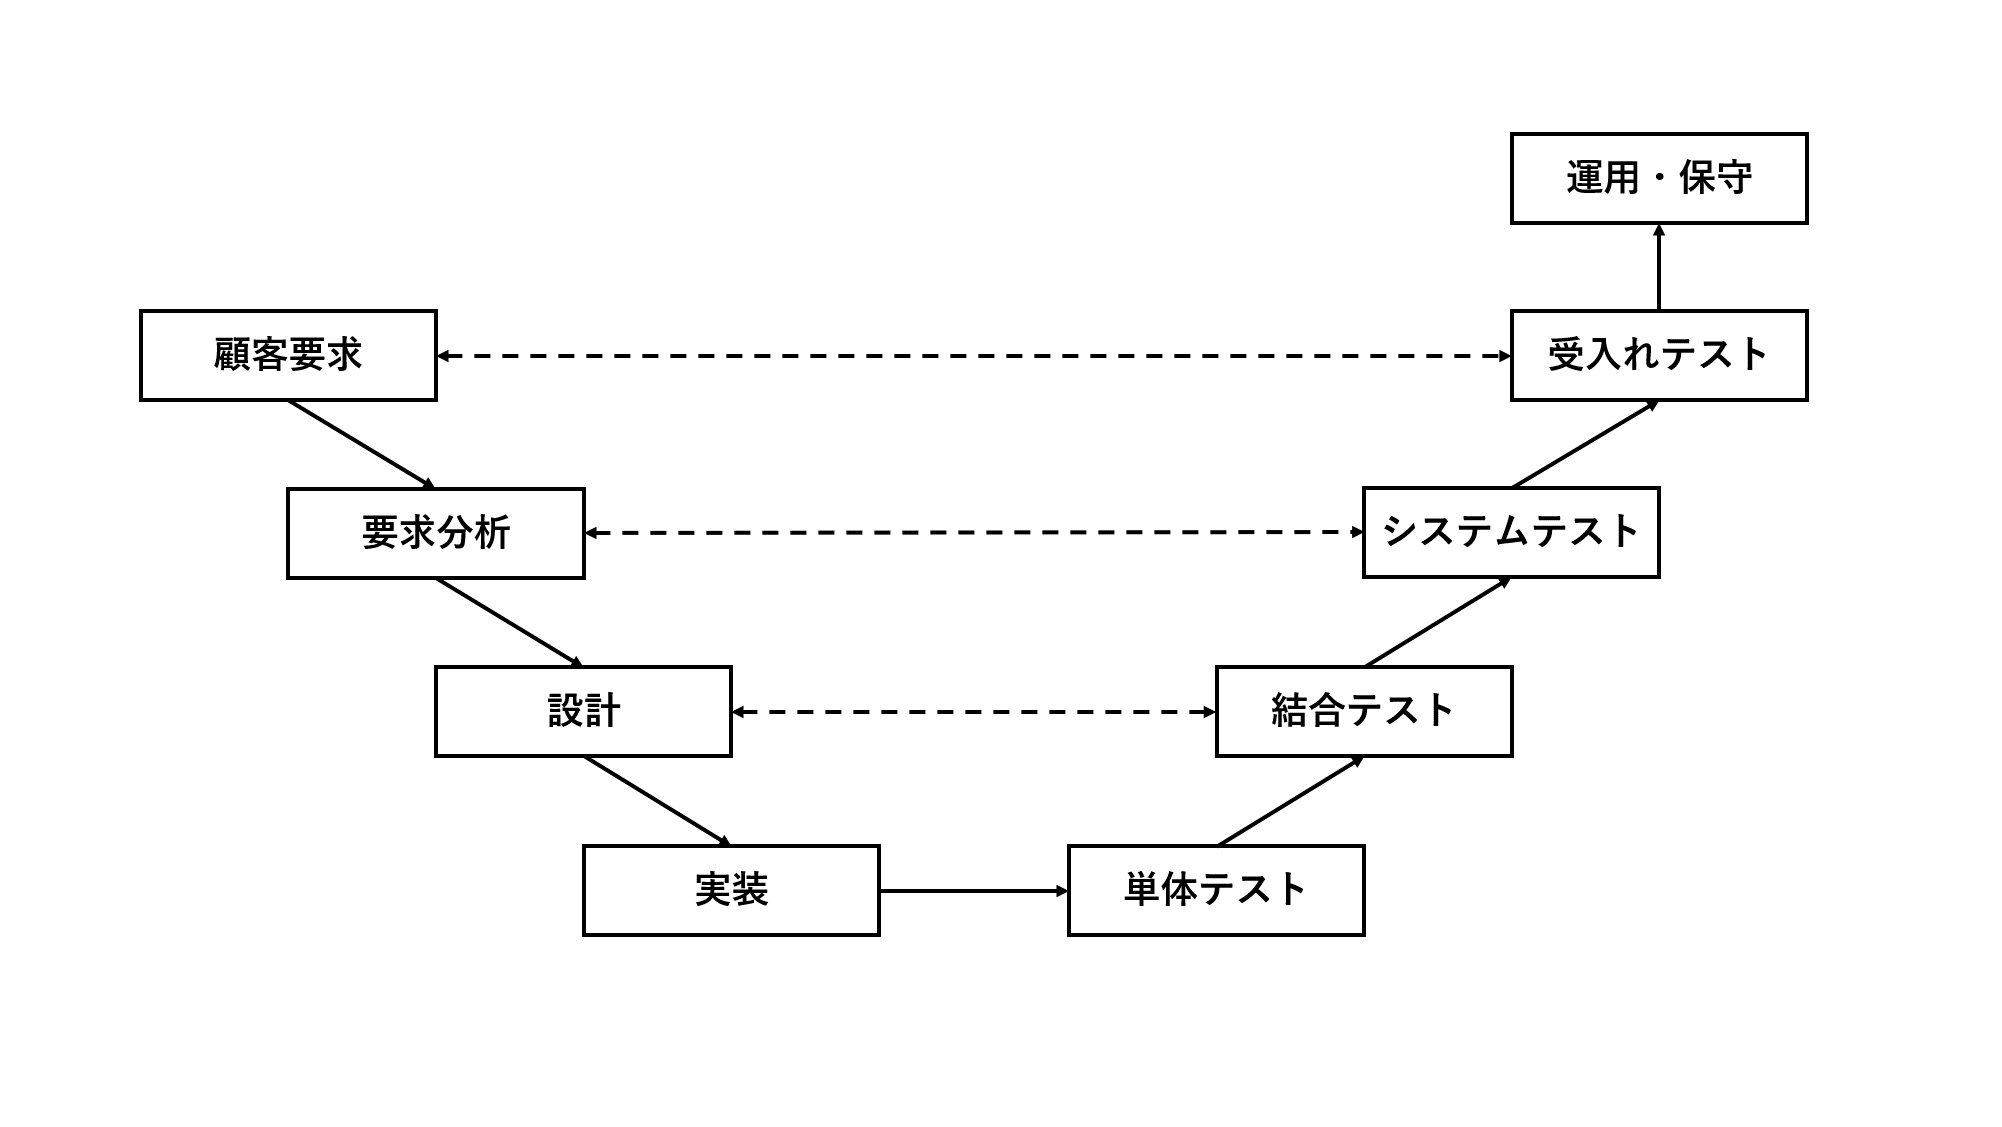
\includegraphics[width=12cm]{buiji.eps}
	\caption{V字モデル}
	\label{buiji}
\end{figure}


\subsection*{UML\cite{uml}}
UMLとは、統一モデリング言語(Unified Modeling Language)のことで、50以上の方法論やダイアグラム表記法のよさをできるだけ踏襲するように共通点を抽出すると同時に、オブジェクト指向でモデリングする際に必要な概念をすべて抽出し、それらを整理統合するような新たなモデル記述体系として考案されたものである。UMLを用いることで対象となる領域やシステムがどのような概念や要素から構成されているかという、構造的な側面のモデル化と、そうした概念や要素が時間経過の中でどのように相互作用して振る舞い、変化を行うかという動的な側面のモデル化の両方を、統一的でビジュアルな言語を使って行うことができる。そのため、組織やプロジェクト固有の慣習を捨象して世界共通の土台で議論できるようになり、計画やコンセプト作りから設計の詳細検討、実装やテストのための仕様定義といった様々な局面で普遍的に活用することができる。本研究でも、開発メンバー4人が1つのチームとして、共通認識を持って開発に取り組むため、要求分析・設計の工程でUML図を作成した。

\subsection*{ユースケース図\cite{uml}}
ユースケース図とは、システムがどのように機能すべきかという振る舞い(ユースケース)と、その外部環境(アクター)を表現するもので、システムの外部と内部との境界を明確にすることができる。ユースケース図を用いることで、エンドユーザの視点からシステムを見ることができ、エンドユーザや領域の専門家とのコミュニケーションが円滑になり、要求に対する相互の理解を保証することができるようになる。

\subsection*{アクティビティ図\cite{uml}}
 アクティビティ図とは、ひとまとまりの業務や処理の内容や流れを表すために、関連する複数の業務手順や処理ステップを順序だてて配置したもので、アクティビティ図によって、「企業全体や業務全体のモデルにおける一連のワークフロー」、「ユースケースごとに対応する処理フロー」、「あるオブジェクトの持つ1メソッドの内部のアルゴリズム」を記述することができる。

\subsection*{クラス図\cite{uml}}
クラス図とは、モデルの静的な構造を表現できる図であり、データ構造(属性リスト)と振る舞い(操作リスト)を持つクラスと、クラス間の静的な関係が表現できる。このクラス図が、UMLに代表されるオブジェクト指向分析設計における中心的な図となり、問題領域の構造や対象システムのアーキテクチャの静的な構成、システムの詳細設計、問題解決の発想の起点となる概念マップの構築といったことに広く用いることができる。

\subsection*{シーケンス図\cite{uml}}
シーケンス図とは、オブジェクト間のメッセージのやり取りを時系列に沿って並べて表現したもので、ユースケースを実現するのに必要なオブジェクトの集合と、その相互作用を明確に表現できる。ここでは、メッセージを時間順に1つずつ記述できるため、シナリオと対応させて具体的な内容を示す際に有用である。


%第3章 
\chapter{感染症予防サポートシステムの設計}
%第3章
本章ではまず、3.1節にて本研究で開発する「感染症予防サポートシステム」の概要を述べる。続いて3.2節ではユースケース図、ユースケース記述を用いて、システムの要求定義について述べる。3.3節ではアクティビティ図、クラス図を用いて、システムの基本設計について述べる。3.4節ではシーケンス図を用いてシステムの詳細設計について述べる。


%第3-1章
\section{感染症予防サポートシステムの概要}
本節では、はじめに感染症予防サポートシステムの開発の目的について説明した後、それを実現するための手段、開発を進める際の課題について述べ、実際に開発したシステムの概要について説明する。

まず私たちは、システムを開発するにあたって、本研究で開発するシステムの目的を定めるところから始めた。何よりもこのシステムで実現しなければならないことをメンバー同士で議論し合った結果、1章で述べたように、世界的な感染拡大が続く新型コロナウイルスへの感染予防対策の一環として取り組むべきとされている、3密の回避のサポートを第一の目的とした。具体的には、学校の教室などの、数人から数十人程度が利用するような部屋で稼働させることで、その部屋に入室可能な人数の目安を示し、部屋の警戒レベル・感染リスクを分析することで、密閉を防ぎつつ、状況に応じて部屋に滞在可能な人数を段階的に制限することによって、その部屋に滞在する人々を3 密の危険から守ることを想定し、システム開発を進めることとなった。続いて私たちは、この目的を実現するためにシステムが果たすべき役割として、以下の2つが挙げられると考えた。


\begin{itemize}
	\item 感染症予防対策のルールを守ってもらうよう働きかける役割
	\item 感染症予防対策の基準を定める役割
\end{itemize}

少なくともこれら2つの役割を満たして、はじめてこのシステムが利用者による3密回避のための行動をサポートできると考えた。3密の回避においては、「密閉」「密集」「密接」の3つの要素が関与することから考えても、上に示した2つの役割を果たすシステムの開発を行うには、その方法を十分に議論する必要があったが、実際の詳細な設計に関しては後で述べる。

続いて本研究で開発するシステムが、先ほど述べた2つの役割を果たすためには、どのような働きを持つべきかを議論した。

まず、利用者に感染症予防対策のルールを守ってもらう役割を果たすには、利用者の感染症予防対策への取り組みの状況を、利用者自身が把握できる必要があると考えた。つまり、リアルタイムで部屋の利用者の感染症予防対策の取り組みを監視し、現在の取り組みがルールに即したものであるかどうかの度合いを知らせ、ルールに反している場合には警告を出すなどし、利用者に感染症予防対策を促すような機能が求められると考えた。

また、感染症予防対策の基準を定める役割を果たすためには、リアルタイムな環境モニタリングによる、総合的な環境分析から得られる結果に基づいた基準を定める必要があると考えた。ここでは、環境の監視と分析の2つの機能が必要となり、環境の監視からどのような情報が得られ、その情報が分析の機能によって、どう意味付けされ、分析の結果得られる情報が感染症予防対策に、どう反映されるべきかを考える必
要がある。

このように、本研究で開発するシステムには、監視と分析という2つの機能が必要になる。これらの機能について、機能を実現する際の方針と課題について述べる。

\subsubsection*{監視の機能}

まず監視の機能については、どのような情報をどのようにして収集するかを考えた。まず3つの密のうち、「密閉」を避けるためには部屋の換気状況を監視する必要がある。こちらは、部屋に人が滞在している状況で、部屋の空気の入れ替えが十分に行われているかどうかを把握できれば良いため、室内の二酸化炭素濃度の高さを監視することによって、状態を把握できると考えた。

ここで考慮しなければならないのが、適切に部屋の換気状況を調べるためには、どのような場所に何台のセンサデバイスを設置すればよいかである。二酸化炭素は気体の一種であるため、部屋中に一様に広がっているわけではなく、同じ部屋の中でも場所によって、微妙に濃度が異なるはずである。したがって、部屋の中心に1台のセンサデバイスを設置しただけでは、室内の二酸化炭素濃度を適切に計測したことにはならないため、部屋の広さに応じてセンサデバイスを、複数台設置する必要があると考えた。ただし、ここで用いるセンサデバイスには、1章でも述べたように無線マイコンモジュールTWELITEを選定した。

「密集」「密接」を避けるためには、部屋に滞在する人の数を監視するだけでなく、部屋の広さに関する情報も必要となると考えた。また、ソーシャルディスタンスを保つために、何平方メートルに1人が滞在可能とするかといった、部屋の運用ルールも併せて考えることが、「密集」「密接」の回避のために扱う情報として適当であると考えられることから、部屋に関する情報も併せて分析の対象とすることとした。

部屋に滞在する人の数に関しては、室内にWebカメラを取り付けたマイコンを設置し、取得した室内画像に対し、物体検出の技術を用いることで、監視することが可能となる。ここで考慮すべき点は、Webカメラによって部屋全体の画像を取得するには、どのようにマイコンを設置しなければならないかという点と、画像識別のプログラム実行にかかる時間によって、監視のリアルタイム性が損なわれないかという点である。今回採用した物体検出の技術による人数推定の方法では、Webカメラによって取得する室内画像が室内全体を捉えていなくてはならない。本システムで想定している利用環境は、学校の教室などであるため、部屋の前方の壁に取り付けるのが、最も部屋全体を捉えるためには適している。反対に、部屋全体を捉えられるような場所にカメラを設置できない場合や、部屋が広すぎるために1台のカメラでは部屋全体を捉えられないという場合には、本システムの運用には適さないということになる。

なお、本システムにおける、物体検出技術による人物の検出機能には、検出精度のみならず、迅速に人物検出の結果を出力することが求められることから、GPUによる高速な処理を可能とする高価なマイコンが必要となる点や、複数箇所から撮影した複数枚の画像から、室内の人数を推定することの技術的な壁の高さから、Webカメラとマイコンの対を、1つの部屋に複数設置するということを本研究では行わない方向となっている。このような点から、本システムを運用する際に推奨される環境としては、数人から数十人程度で使われる、比較的小さな部屋で、なおかつ設置したカメラによって部屋全体を撮影できることが条件となる。ただし、ここで用いるマイコンには、1章でも述べたようにAIエッジ向けコンピュータとして知られるJetsonシリーズのJetson nanoを選定した。

\subsubsection*{分析の機能}

分析の機能に関しては、監視によって得られた情報から、より高い価値を持つ「感染予防対策に役立てられる情報」を導き出すための分析方法を議論した。

分析の機能でははじめに、二酸化炭素濃度の高さから、部屋の感染症に対する警戒レベルを導出する。二酸化炭素濃度が高くなるほど、部屋が密閉された状態になっていると考えられるため、部屋の警戒レベルは高く設定される。ここで考慮しなくてはならないのが、ある時間に取得した二酸化炭素濃度だけで部屋の換気状態を正しく分析できるかという点であり、データに多少のばらつきがみられる可能性から考えて、一定時間連続的に取った値をもとにして分析を行う必要があると考えた。

続いて、導出された警戒レベル毎に制限される、室内に滞在可能な人数と、実際に室内に滞在している人数とを比較し、感染リスクを導出する。警戒レベル毎の滞在可能人数には、上限と下限を設け、上限を超える場合には感染リスクが最高となり、下限から上限の範囲内であれば、室内の滞在人数を維持できるものとし、下限を下回る場合には、感染リスクを高めない範囲内で滞在人数を増やすことができる段階にあるものとして、3段階で感染リスクを評価する。ただし、警戒レベルの高さに関わらず、部屋の広さと部屋の運用ルールから求められる部屋の滞在可能規定人数を上回る場合には、感染リスクは最高となる。

このようにして、分析の機能では、室内環境の監視によって得られた情報をもとに、部屋の警戒レベルと感染リスクを評価する。

ここまで、本研究で開発するシステムの目的、機能を実現する際の方針と課題について述べてきた。ここからは、実際に開発したシステムの概要を説明する。

まず、本研究で開発するシステムを利用する際の簡単な流れを図\ref{systemflow}に示す。

\begin{figure}[H]
	\centering
	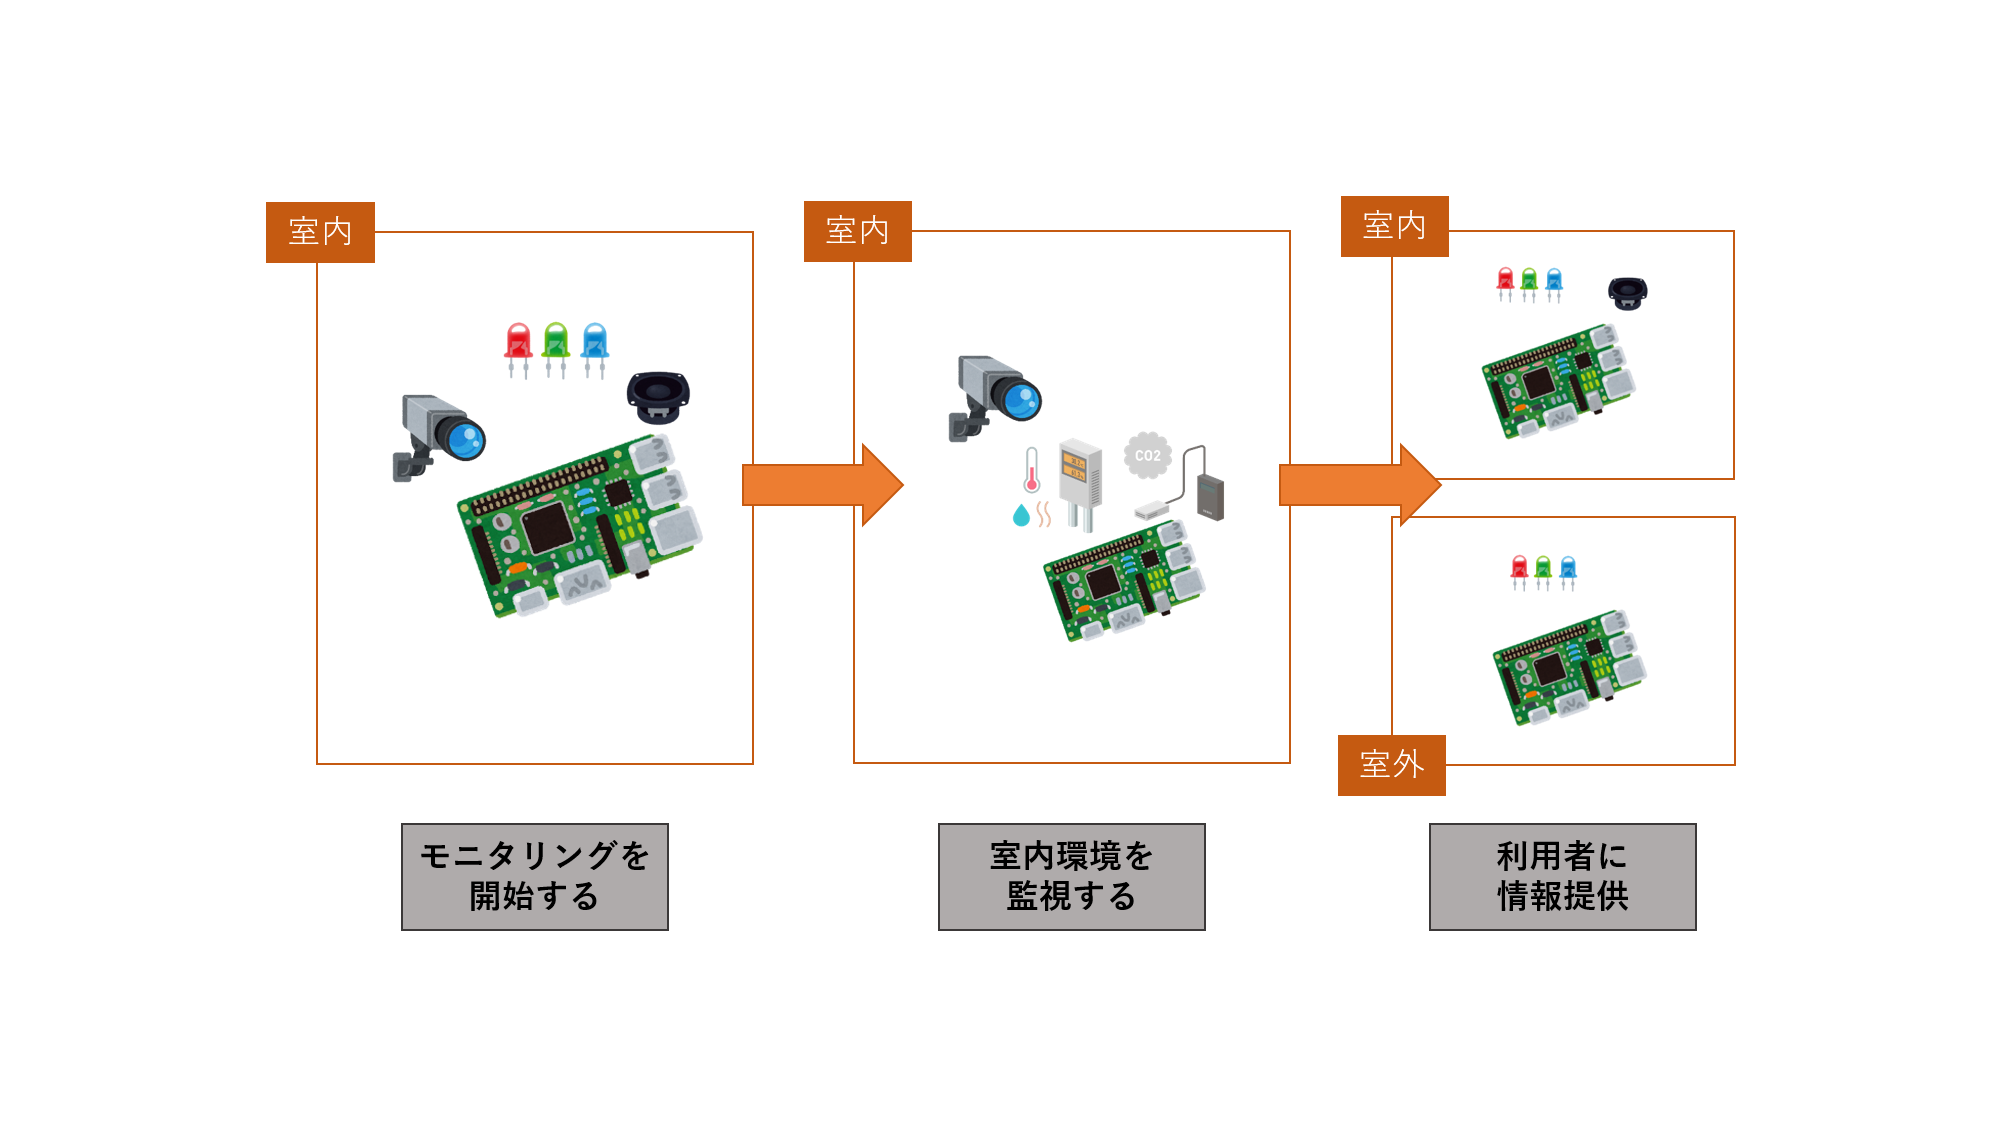
\includegraphics[width=15cm]{systemflow.eps}
	\caption{システム利用の流れ}
	\label{systemflow}
\end{figure}

まず、利用者はエッジサーバとしてシステム全体の中心となって稼働するJetson nanoに、部屋情報として、部屋の広さと何平方メートルに1人が滞在できるかという、部屋の運用ルールを登録する必要がある。感染予防サポートシステムを稼働させるには、このJetson nanoと、センサデバイスとして用いるTWE-LITEを室内に設置する。センサデバイスは部屋の広さなどに応じて、台数を増やすことが可能である。また室外には、部屋への入室の危険度を知らせるためのデバイスとして用いるTWE-LITEを設置する。あとは各デバイスの電源を入れ、エッジサーバであるJetson nanoによってモニタリングを開始するのみである。

デバイス類はシステム稼働後にそれぞれ接続され、基本的には3分おきに室内画像と、二酸化炭素濃度や温湿度といった環境値をそれぞれ、Jetson nanoに取り付けたWebカメラ、室内センサデバイスに取り付けたセンサ類によって取得し、それらのデータをJetson nanoで受け取った後、室内画像をもとにした人数推定と環境値をもとにした分析を行う。Jetson nanoでは、分析結果に基づき、換気要請や感染リスク状況をブザーとLEDを用いて、室内の利用者に通知する。また室外デバイスでは、Jetson nanoにより分析された部屋への入室危険度を受け取り、その都度リスクに応じたLEDを点灯する。これら一連の流れを8時から20時まで行い、夜間はスリープ状態に入るというのが、基本的なシステムの稼働の流れである。ここでシステム全体構造のイメージを図\ref{systemconst}に示す。

\begin{figure}[H]
	\centering
	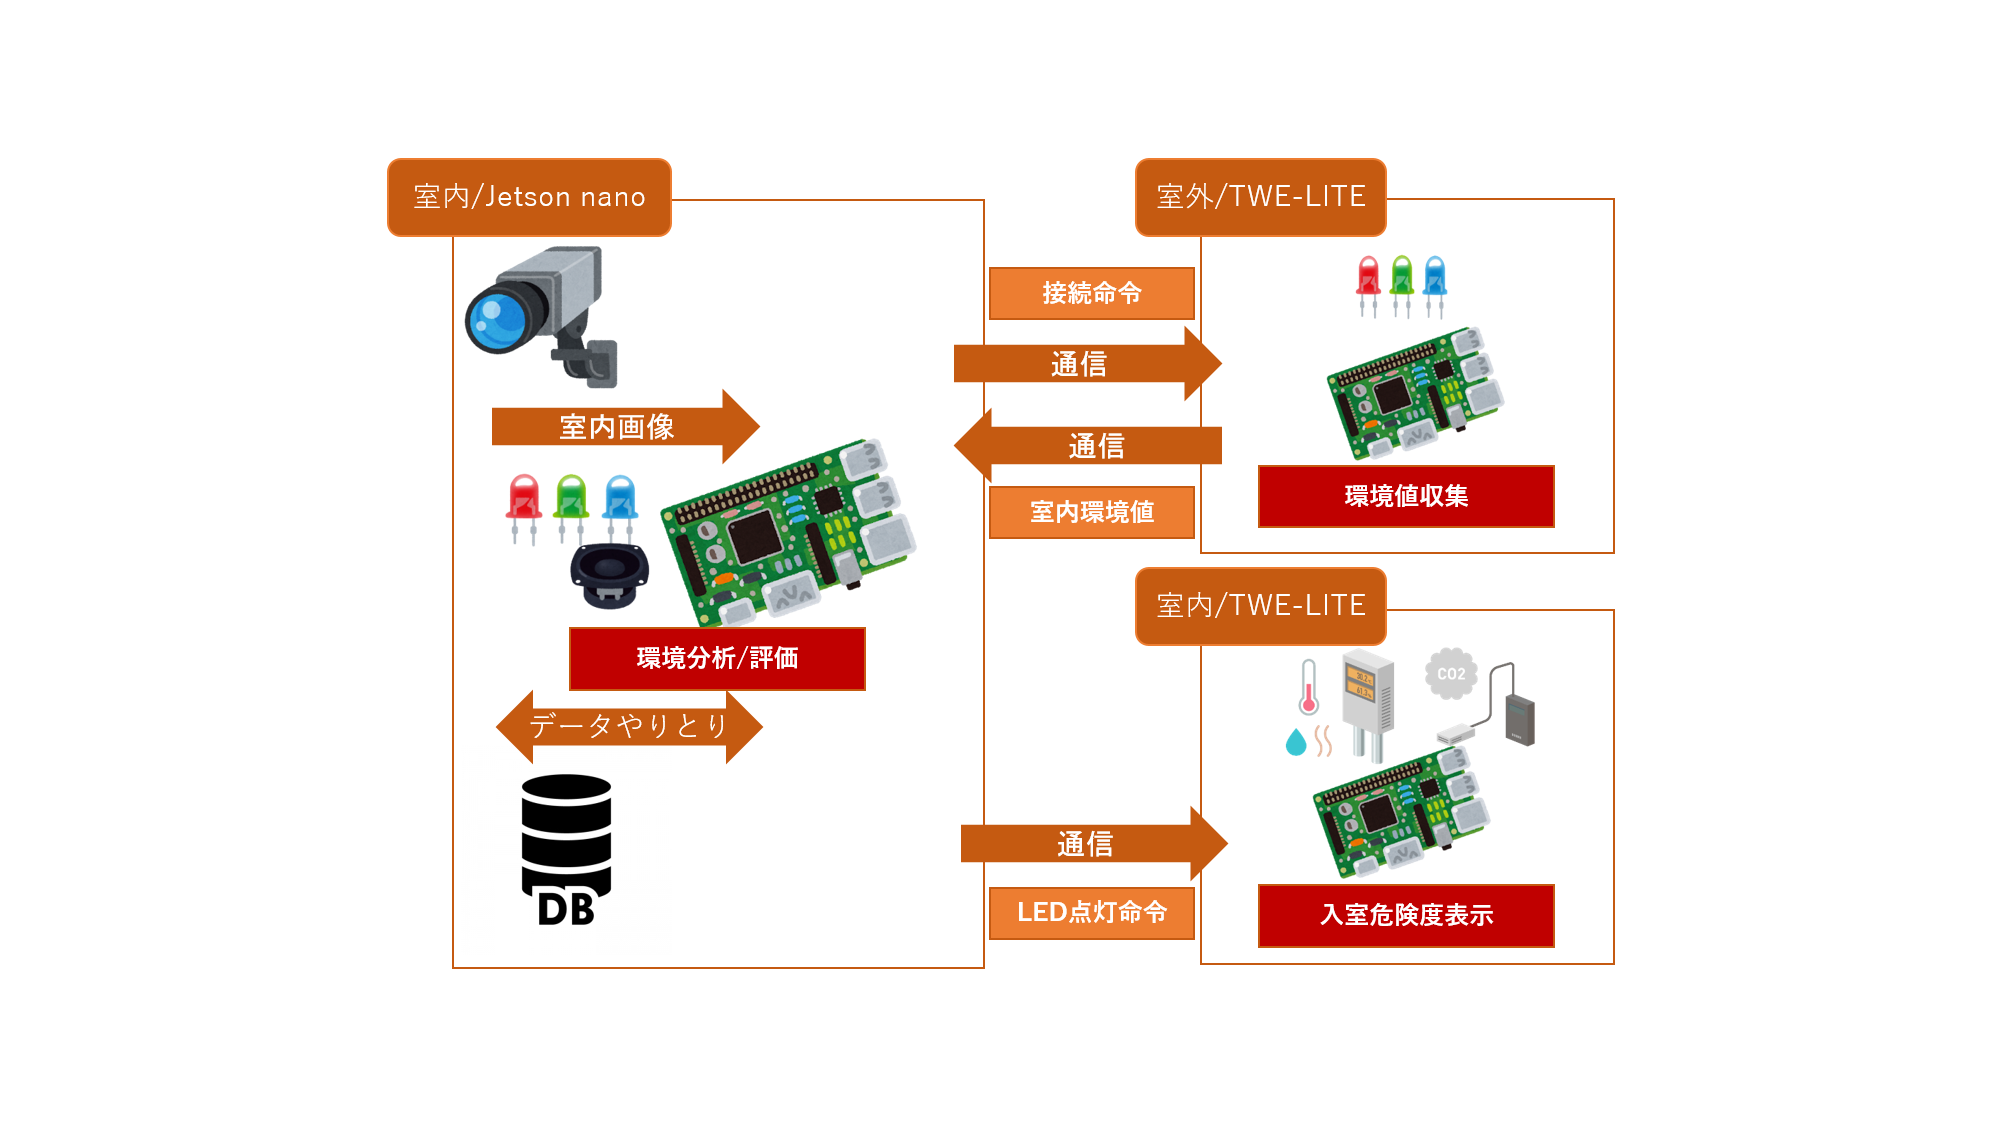
\includegraphics[width=15cm]{systemconst.eps}
	\caption{システム全体構造}
	\label{systemconst}
\end{figure}

なお本システムの開発は、エッジサーバ側を掛水誠矢が、センサデバイス側を稲田一輝が、室外デバイス側を小田恵吏奈が、人数推定機能を伊藤大輝が担当する。




%第3章

\section{要求定義}

感染症予防サポートシステムがどのような機能を持ち,どのような振る舞いをするかを表すために以下の図\ref{usecase1}に示すユースケース図を作成した.

\begin{figure}[htbp]
\centering
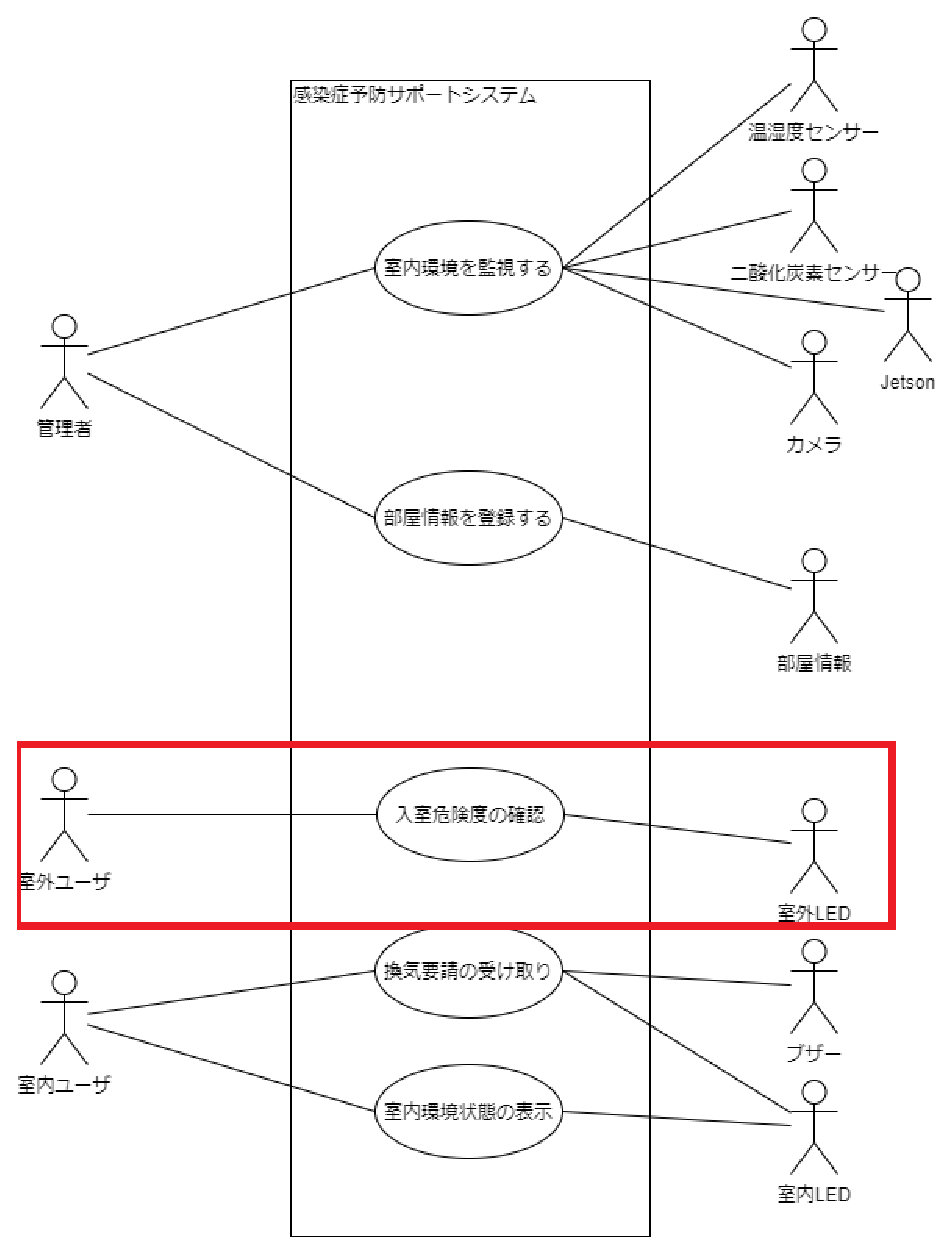
\includegraphics[width = 10cm]{./uml/usecase_e.eps}
\caption{ユースケース図}
\label{usecase1}
\end{figure}

感染症予防サポートシステムの各ユースケースについて述べる.
「室内環境を監視する」では,Webカメラにより取得した画像について人数推定を行い,室内人数に応じた監視モードを開始する.監視モードで測定した二酸化炭素濃度に応じて警戒レベルを設定し,必要に応じて換気要請を出すなどの対応をとる.
「部屋情報を登録する」では,管理者が登録した,システムを運用する部屋の広さを元に,標準警戒レベルでの滞在可能上限人数を定める.
「入室危険度の確認」では,部屋の滞在可能上限人数と現在の室内人数に応じた入室危険度を表す室外デバイスのLEDを点灯する.
「換気要請の受け取り」では,二酸化炭素濃度が各警戒レベルでの基準値を一定時間連続で超えると,LEDやブザーによって換気要請が出され,室内のユーザーは要請に従い換気を行う.
「室内環境状態の表示」では,温湿度の一定時間ごとの測定値を元に室内環境を分析し,温湿度が基準値を超えている場合は室内のLEDが点灯する.これを受けた室内のユーザーは,エアコン等により温湿度の調整を行う.
特に赤枠で囲んだ「入室危険度の確認」は筆者が実装を担当する部分となる.

上記のユースケースを受け,表\ref{sougoutestkoumoku}に示す総合テストの項目を挙げた.

\begin{table}
	\centering
	\caption{総合テスト項目}
	\label{sougoutestkoumoku}
	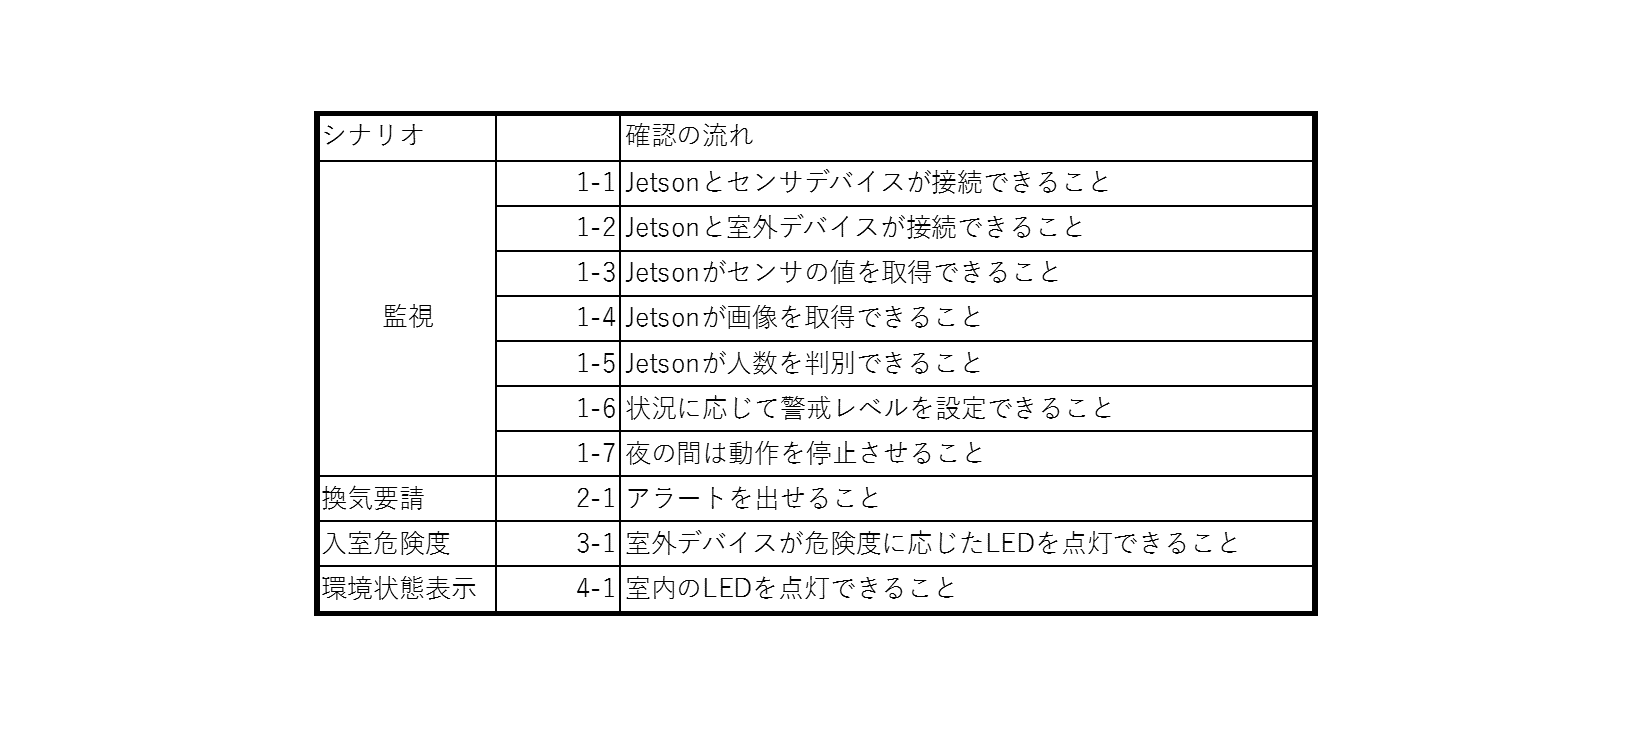
\includegraphics[width=0.9\linewidth]{test/sougoutest_koumoku}
\end{table}
\newpage
%第3-3章
\section{基本設計}
基本設計では、ひとまとまりの処理の内容の流れを表現するために用いるアクティビティ図を作成し、「室内環境を監視する(図\ref{a_kansi})」、「換気要請の受け取り(図\ref{a_kanki})」、「入室危険度の確認(図\ref{a_nyuusitu})」、「室内環境状態の表示(図\ref{a_situnaikankyou})」の4つのユースケースについて、簡単に処理の流れを確認した。以下に作成したアクティビティ図を示す。


\begin{figure}[H]
	\centering
	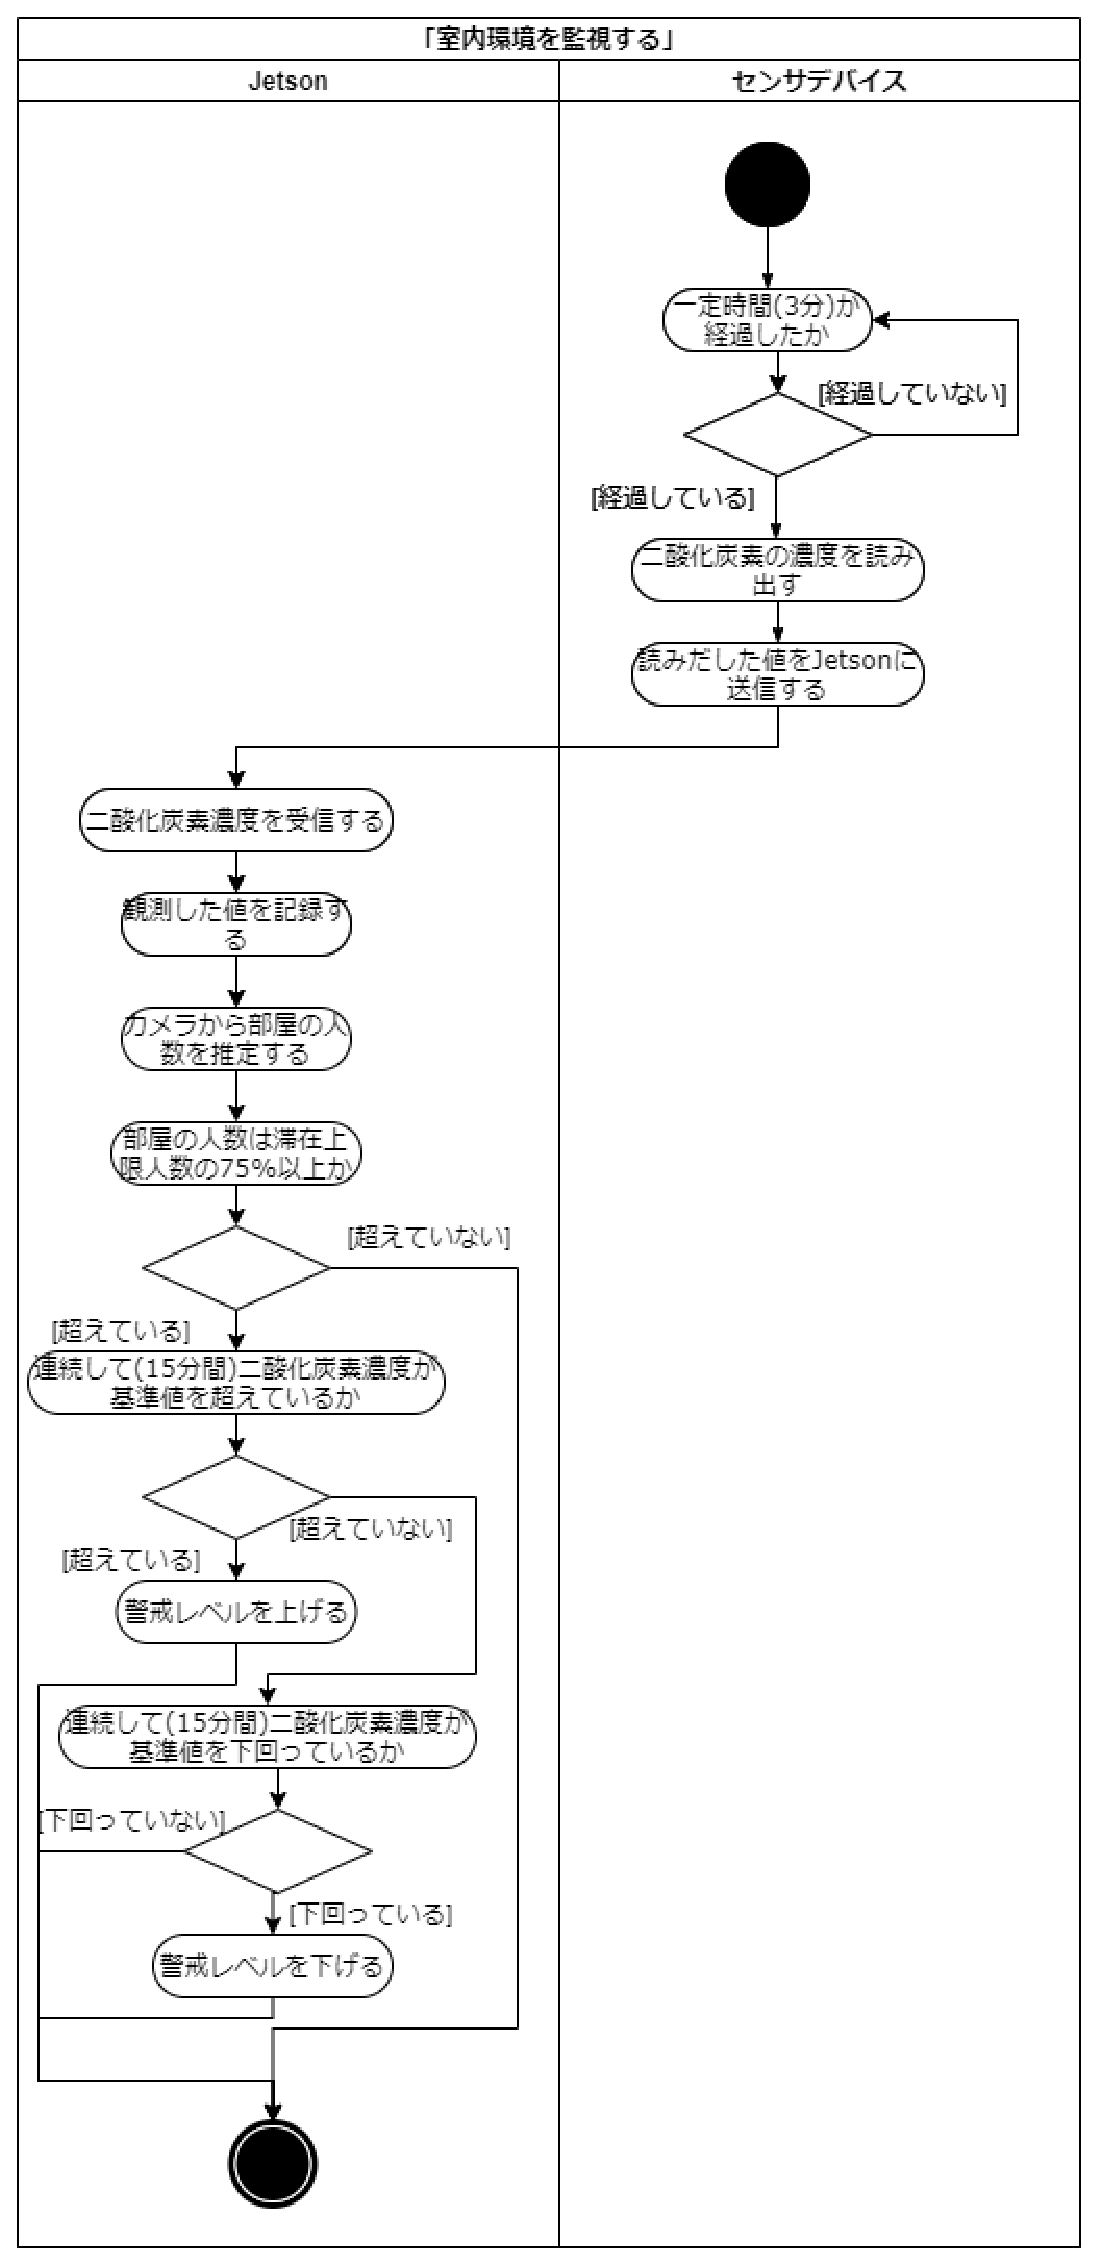
\includegraphics[width=9.5cm]{a_kansi.eps}
	\caption{室内環境を監視する}
	\label{a_kansi}
\end{figure}

\begin{figure}[H]
	\centering
	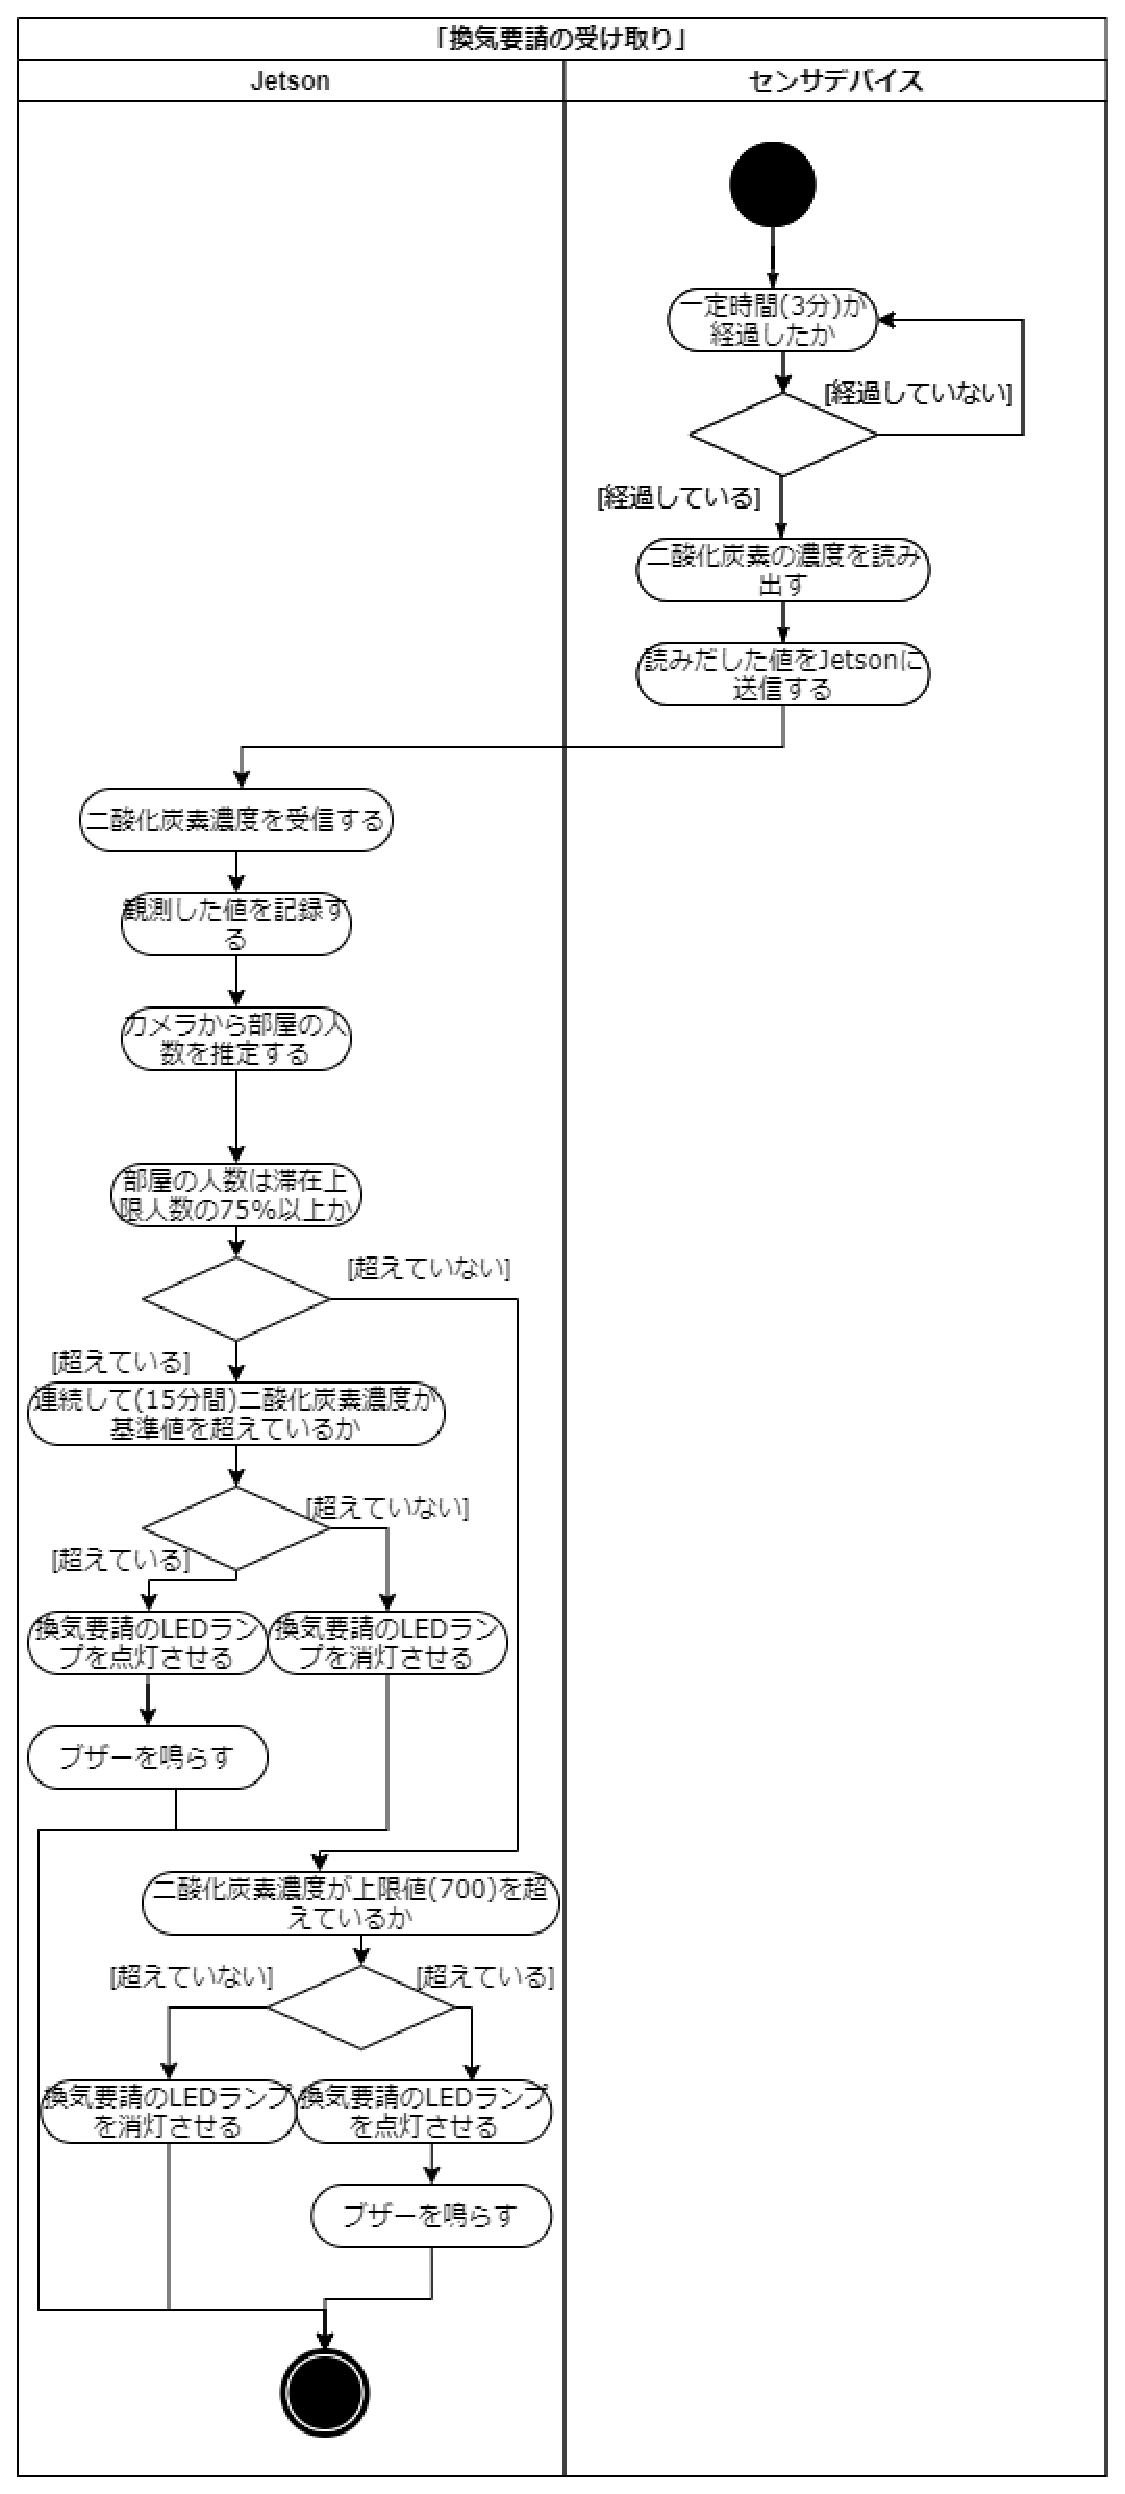
\includegraphics[width=9.0cm]{a_kanki.eps}
	\caption{換気要請の受け取り}
	\label{a_kanki}
\end{figure}

\begin{figure}[H]
	\centering
	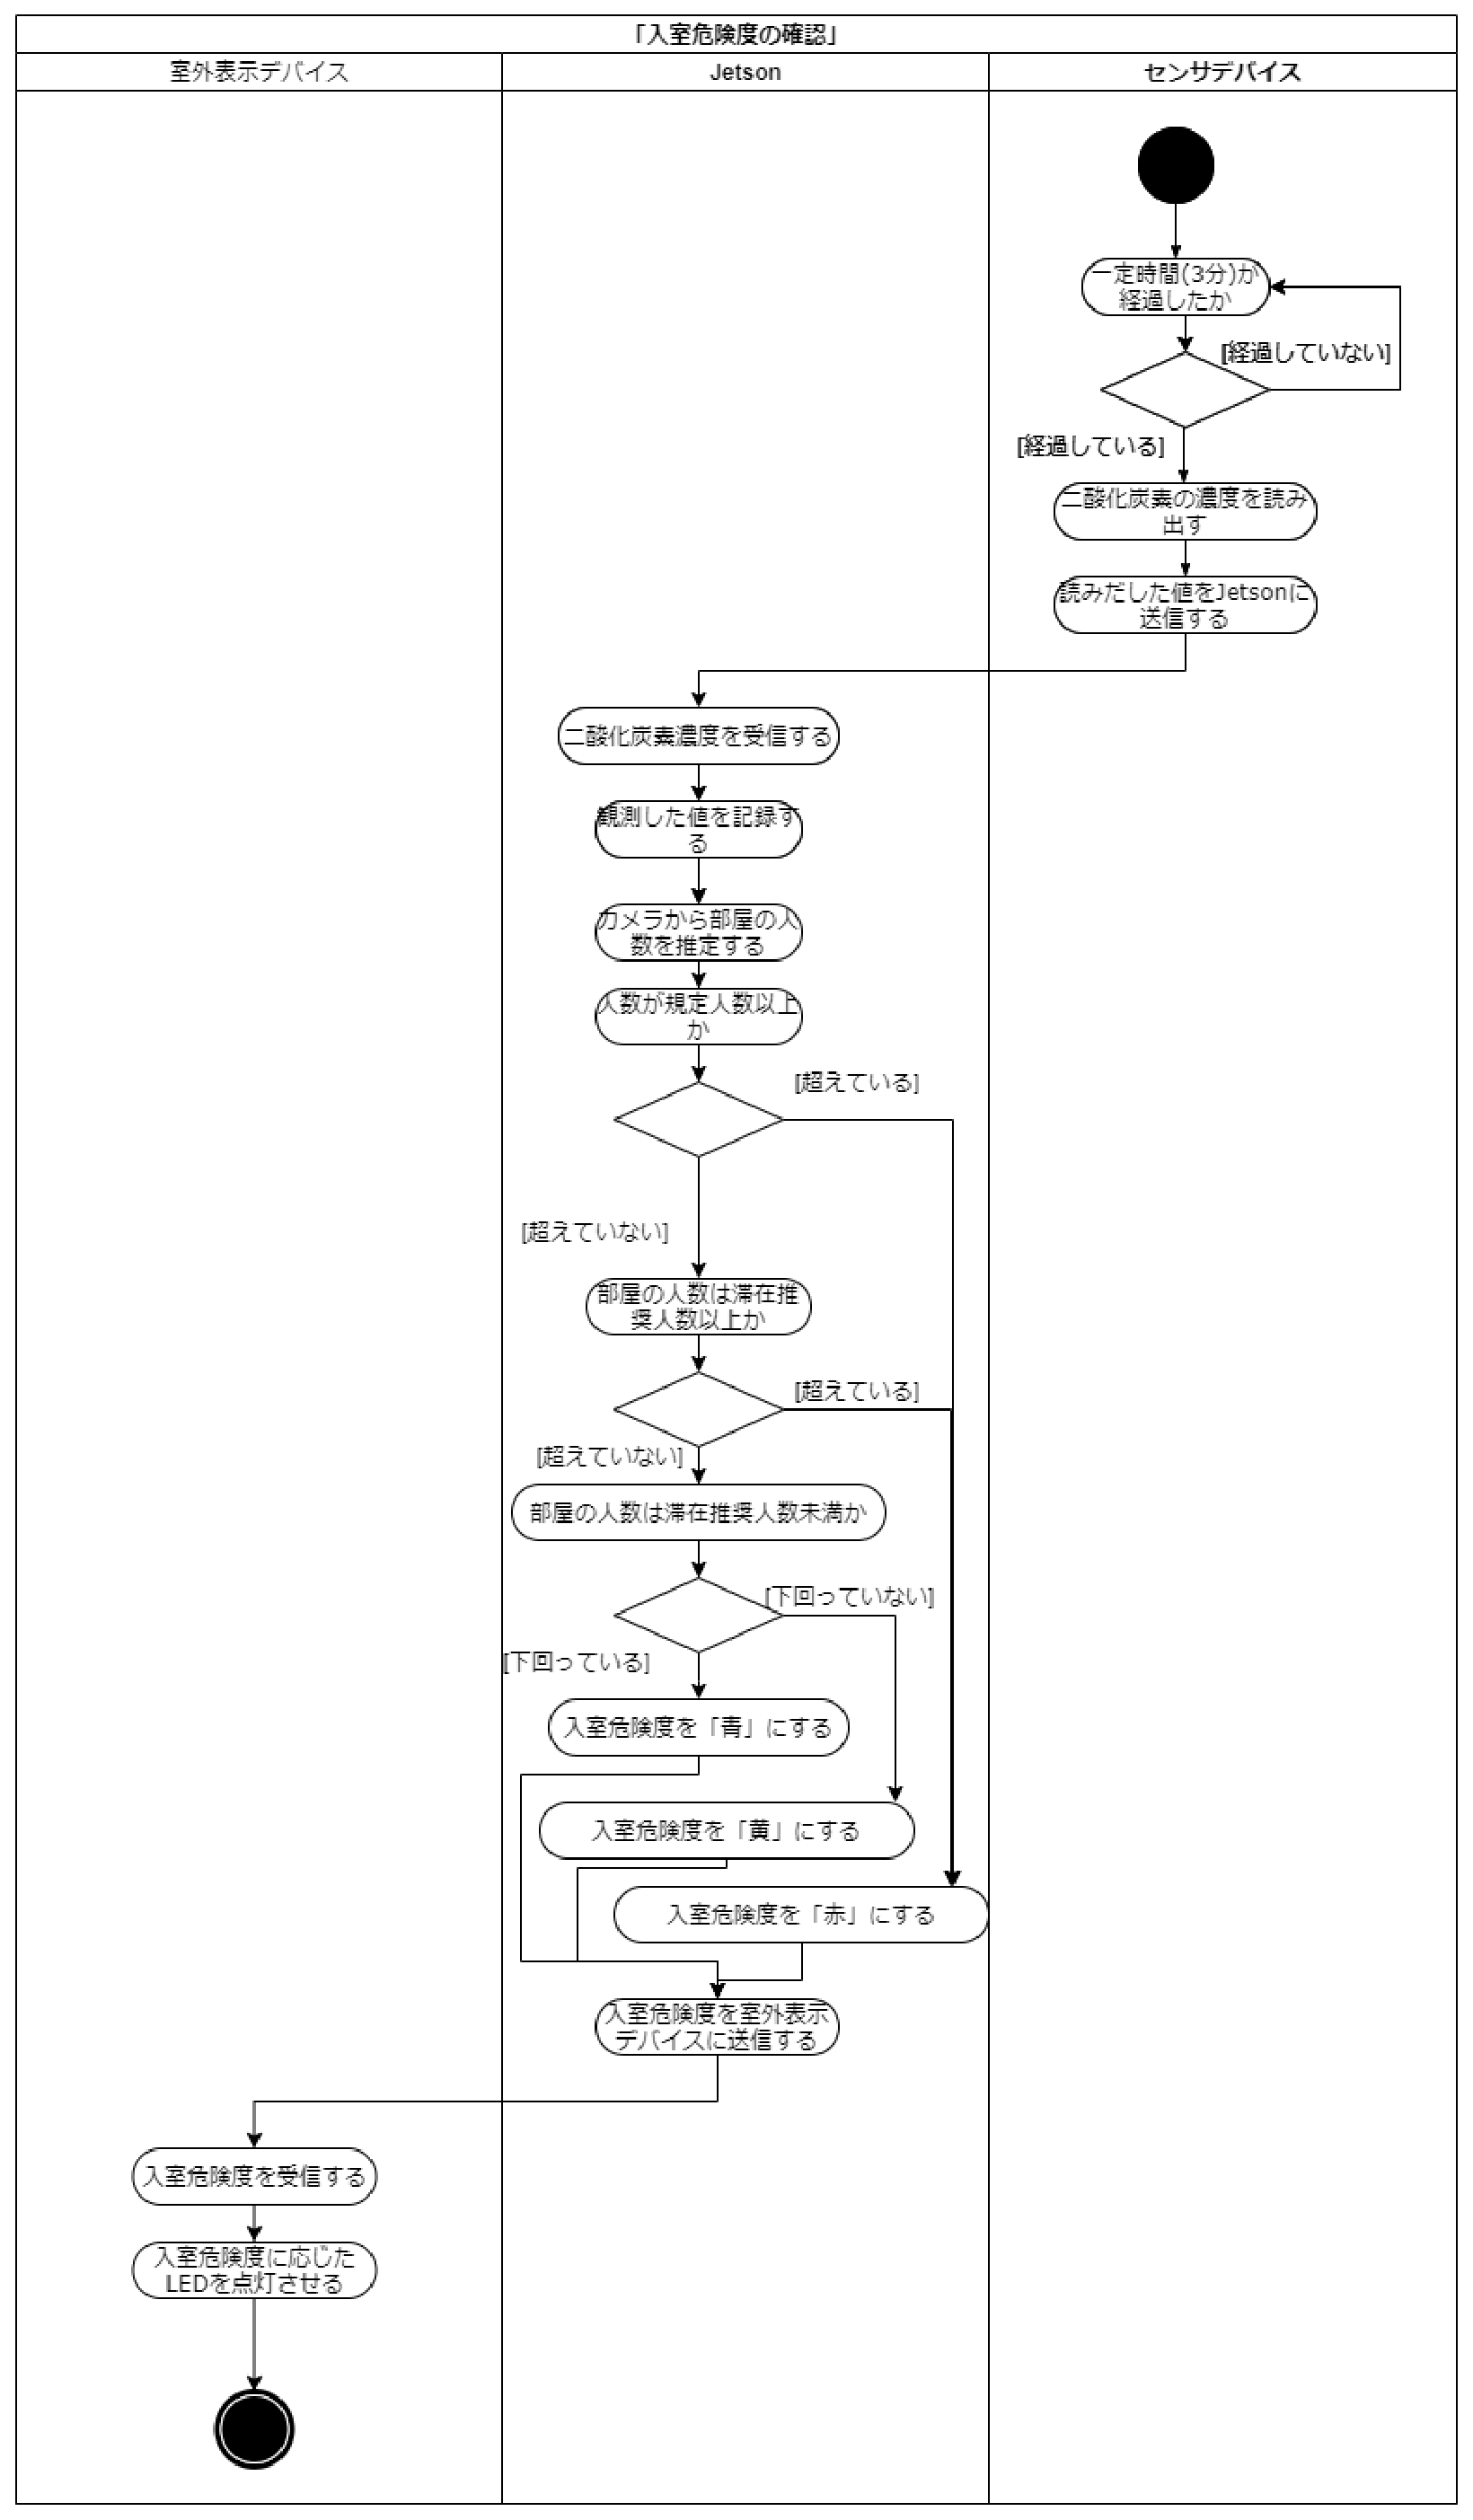
\includegraphics[width=9.5cm]{a_nyuusitu.eps}
	\caption{入室危険度の確認}
	\label{a_nyuusitu}
\end{figure}

\begin{figure}[H]
	\centering
	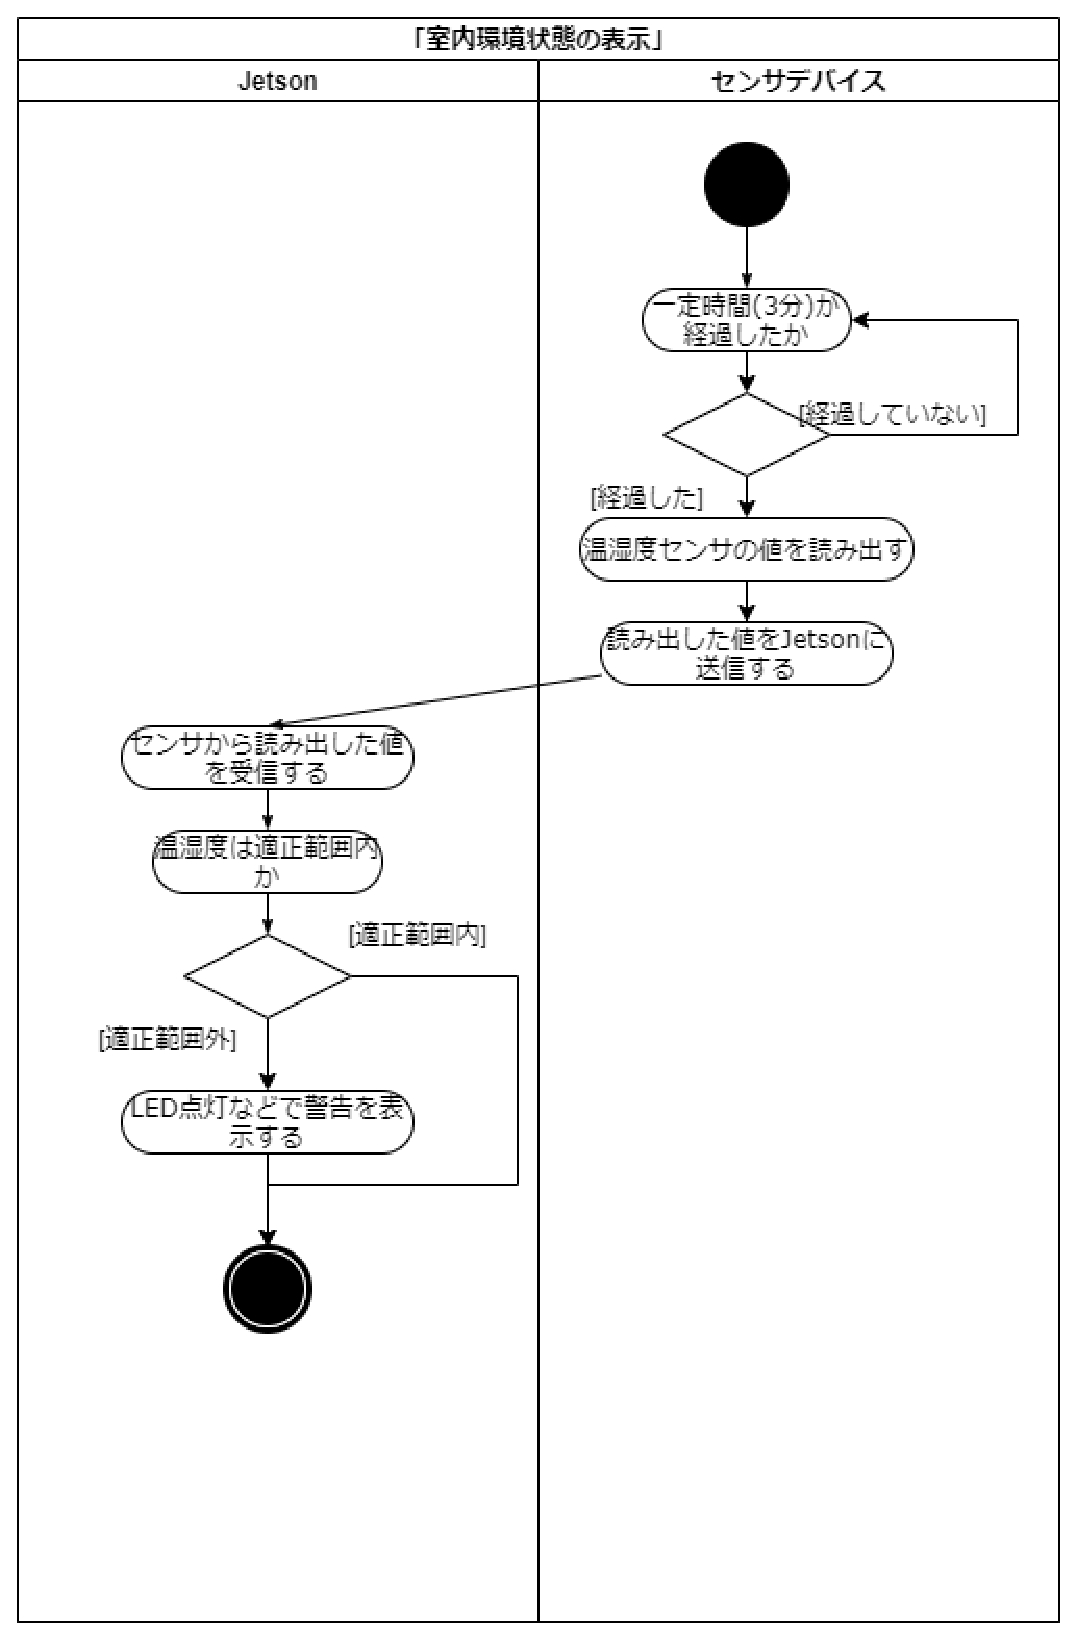
\includegraphics[width=10cm]{a_situnaikankyou.eps}
	\caption{室内環境状態の表示}
	\label{a_situnaikankyou}
\end{figure}

以上の4つのアクティビティ図の作成を通して、それぞれのユースケースを実現する際の処理の流れを可視化することができた。この作業を通して、ユースケース図やユースケース記述を作成した時点よりも、より論理的にシステム内部の設計を進めることができた。

上に示したアクティビティ図では、各デバイスなどのオブジェクトごとの処理のまとまりを、縦の線によってレーンとして明示的に分けて表現している。これによって、各ユースケースの全体的な処理の流れだけでなく、各ユースケースにおいて、処理やデータがオブジェクト間でどのように移されるかを確認することもできた。

具体的に見てみると、室内の複数箇所に設置するセンサデバイスは、センサから値を取得した後は、送信の機能を基本として動作すればよいことが確認できた。一方、Jetson nano側に着目すると、センサデバイスからのデータの受け取りと、室外の入室危険度表示デバイスへのデータの受け渡しというデータの流れが必要となることが確認され、Jetson nano側ではデータの送受信両方の役割を持たせなければならないことが確認できた。また、室外の入室危険度表示デバイス側は、データの取得・分析後の成果物の情報といえる、入室危険度の受け取りさえできればよいということから、受信の機能を基本として動作すればよいことを確認することができた。

アクティビティ図作成の段階では、まだ詳細な処理の流れが示されていないものの、ユースケースを実現する際の大まかな処理とデータの流れを確認することができた。また、この後の詳細設計を進める際にも、ここで作成したアクティビティ図が、基本的な考え方として活かされた。

基本設計の段階では、各デバイスがどのような振る舞いをするかを確認することができたことで、実際にシステムに用いるデバイス類の選定が可能となった。ここまでに、人数推定の機能をリアルタイム性の高い物体検出によって実現するという点から、エッジサーバ側にはJetson nanoを用いることが決まっていたが、この段階でセンサデバイス、室外の入室危険度表示デバイスに用いるデバイス類を決定した。

3.1節でも述べたが、センサデバイスは室内の複数個所に設置することを想定しており、電源の供給方法による取り付け場所の制約を受けず、なおかつ比較的低い消費電力での稼働を可能とするデバイスを選ぶ必要があった。このことから単4乾電池2本で動作し、ワイヤレスセンサーネットワークの構築に適した無線規格であるIEEE802.15.4を採用し、低消費電力での無線通信を可能にする無線マイコンモジュールとしてTWELITEを選定し、室外に設置する部屋への入室の危険度を表示するデバイスに関しても、同じくTWELITEを選定した。また、Jetson nanoにもこのTWE-LITEをUARTによって接続し、センサデバイスとしてのTWE-LITEや、室外の入室危険度表示デバイスとしてのTWE-LITEそれぞれとの通信を可能とし、エッジサーバとして必要となる、データ送受信の機能を持たせている。

ここまでの設計内容をもとにクラス図を作成したところ、図\ref{class}のように本システムの静的な構造が確認できた。ただし、3.4節でも述べるがJetson nano側では、センサデバイスから受け取ったデータを管理するために、データベースを用いることとしている。

\begin{figure}[H]
	\centering
	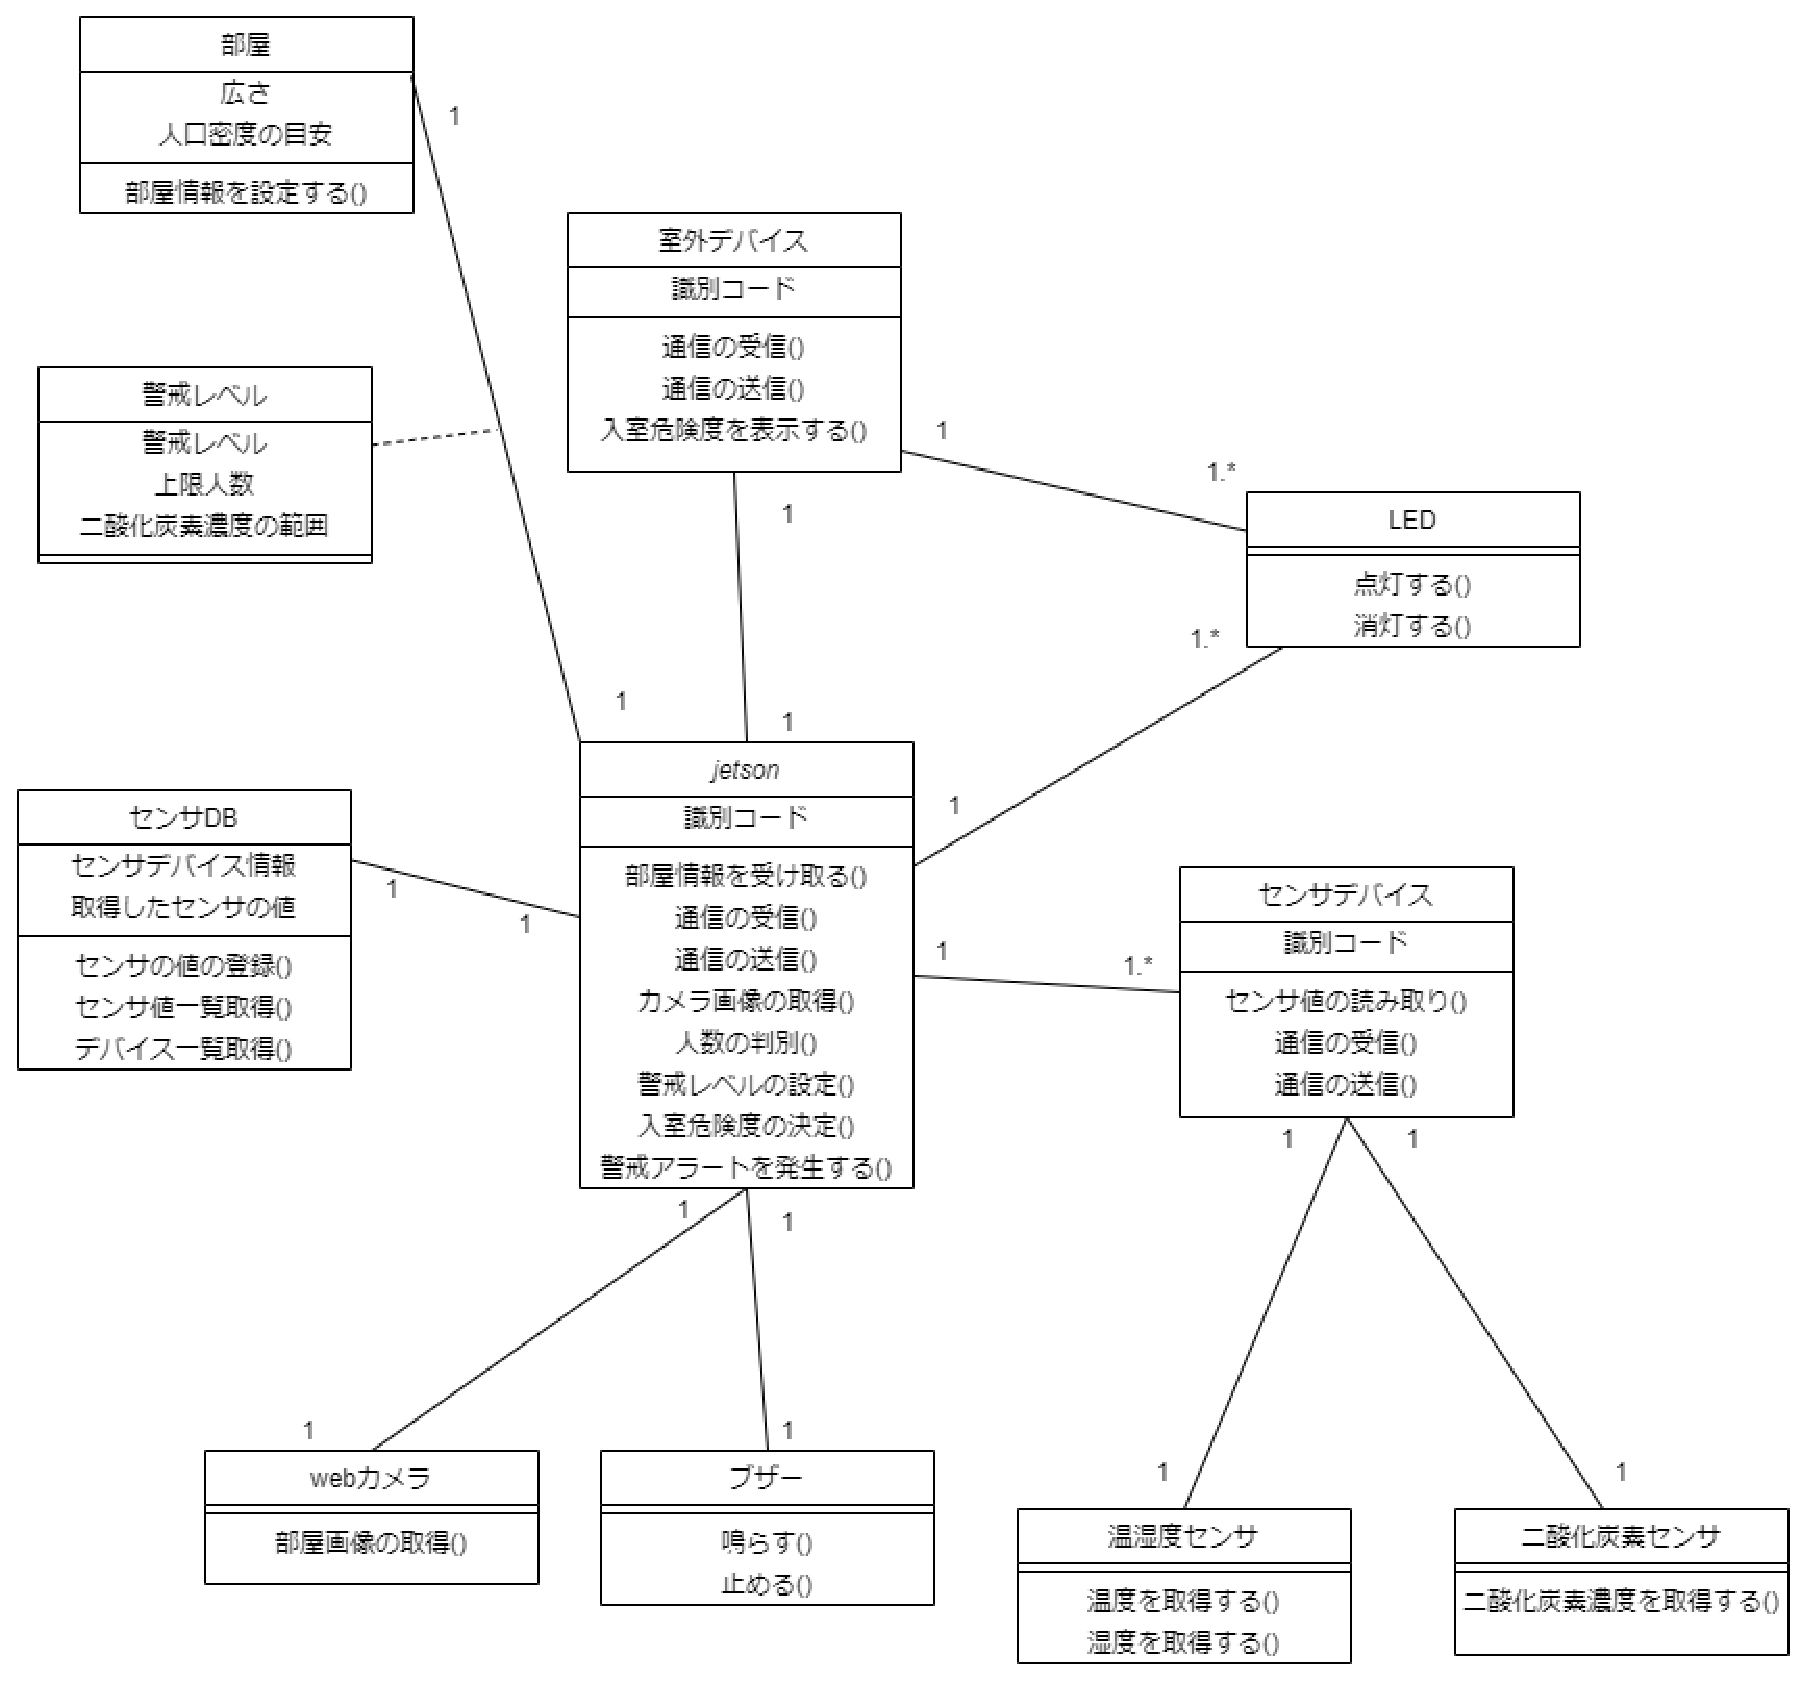
\includegraphics[width=12cm]{class.eps}
	\caption{クラス図}
	\label{class}
\end{figure}


また、以上の基本設計の内容をもとに、結合テスト項目として表\ref{ketugoutest_koumoku}の項目を挙げた。


\begin{table}[H]
	\centering
	\caption{結合テスト項目}
	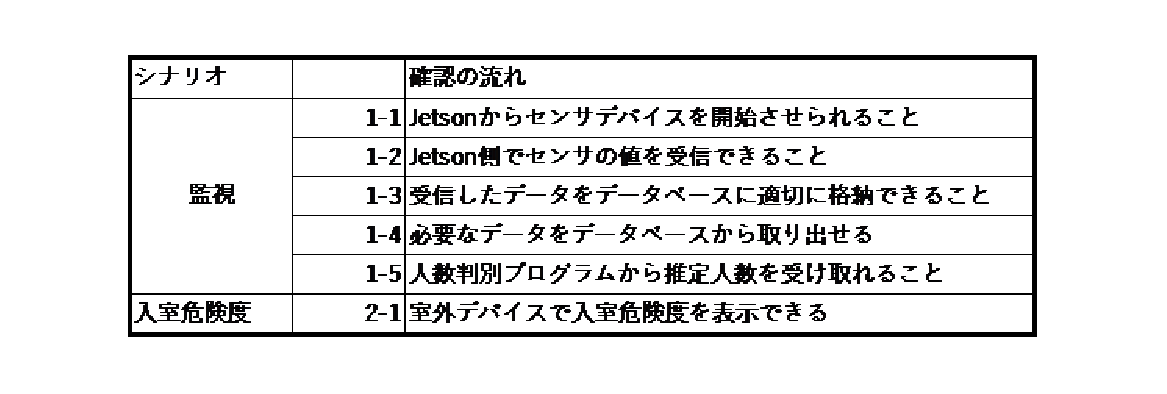
\includegraphics[width=15cm]{ketugoutest_koumoku.eps}
	\label{ketugoutest_koumoku}
\end{table}




%第3章
%図をすべて変更する必要があり

\section{詳細設計}

本節では感染症予防サポートシステムにおける詳細な動作,詳細設計について述べる.

まず,オブジェクト間のメッセージのやりとりを中心に,詳細な動作をシーケンス図を用いて説明する.
「室内状況を監視する」シーケンス図を図\ref{seq_kanshi}に,
「入室危険度の確認」のシーケンス図を図\ref{seq_enterlisk}に,
「換気要請の受け取り」のシーケンス図を図\ref{seq_kanki}に,
「室内環境状態の表示」のシーケンス図を図\ref{seq_kankyou}に示す.
\begin{figure}[htbp]
    \centering
    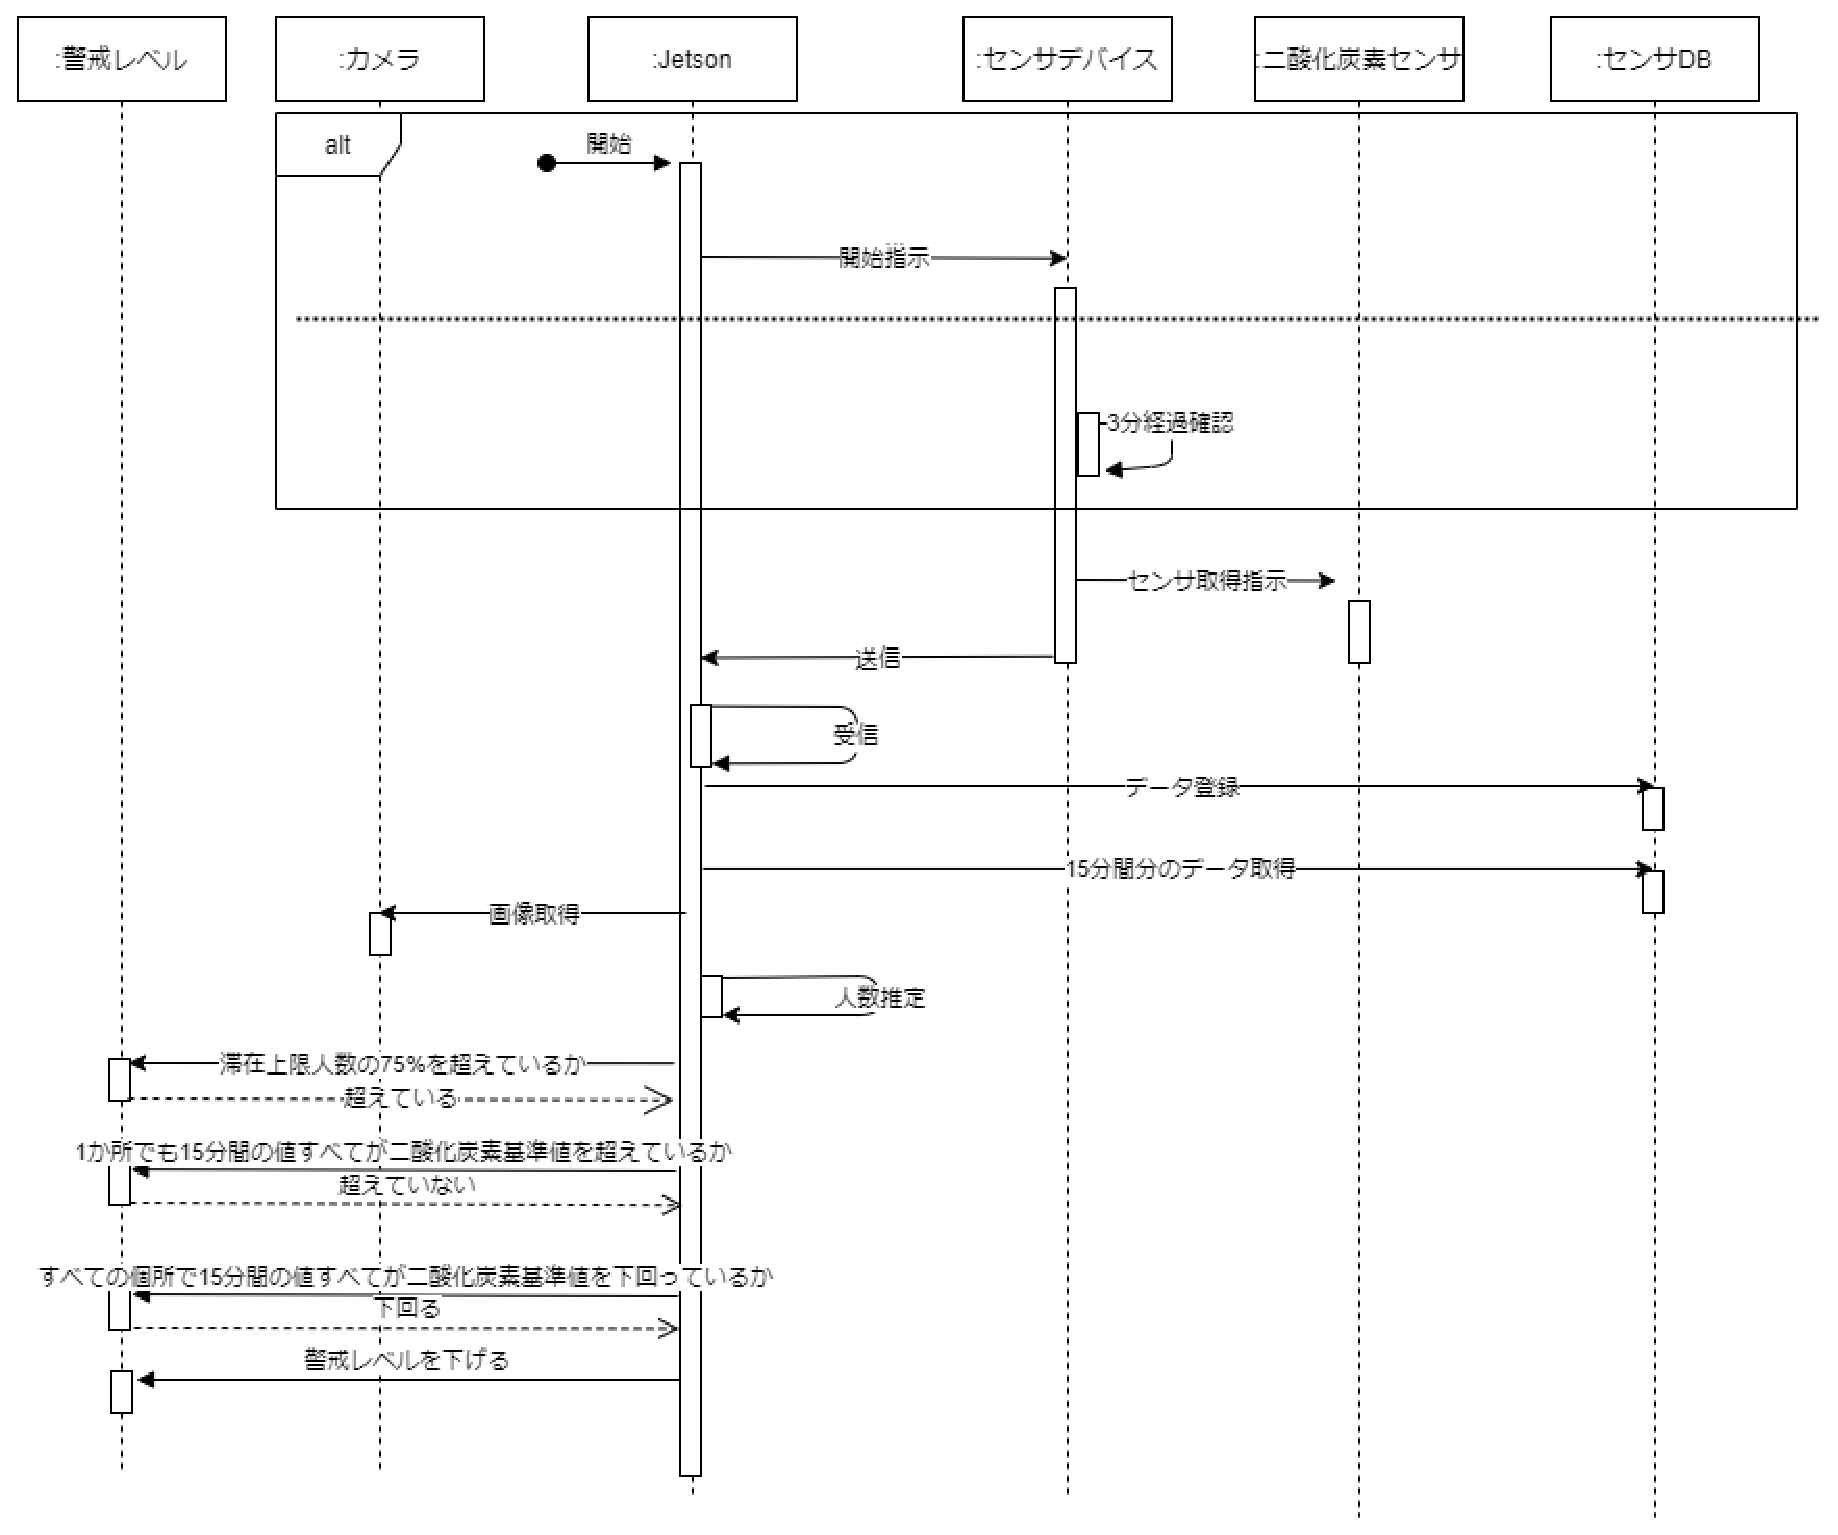
\includegraphics[width = 15cm]{./picture/sequence_kanshi_3.eps}
    \caption{ユースケース「室内状況を監視する」のシーケンス図}
    \label{seq_kanshi}
\end{figure}
\begin{figure}[htbp]
    \centering
    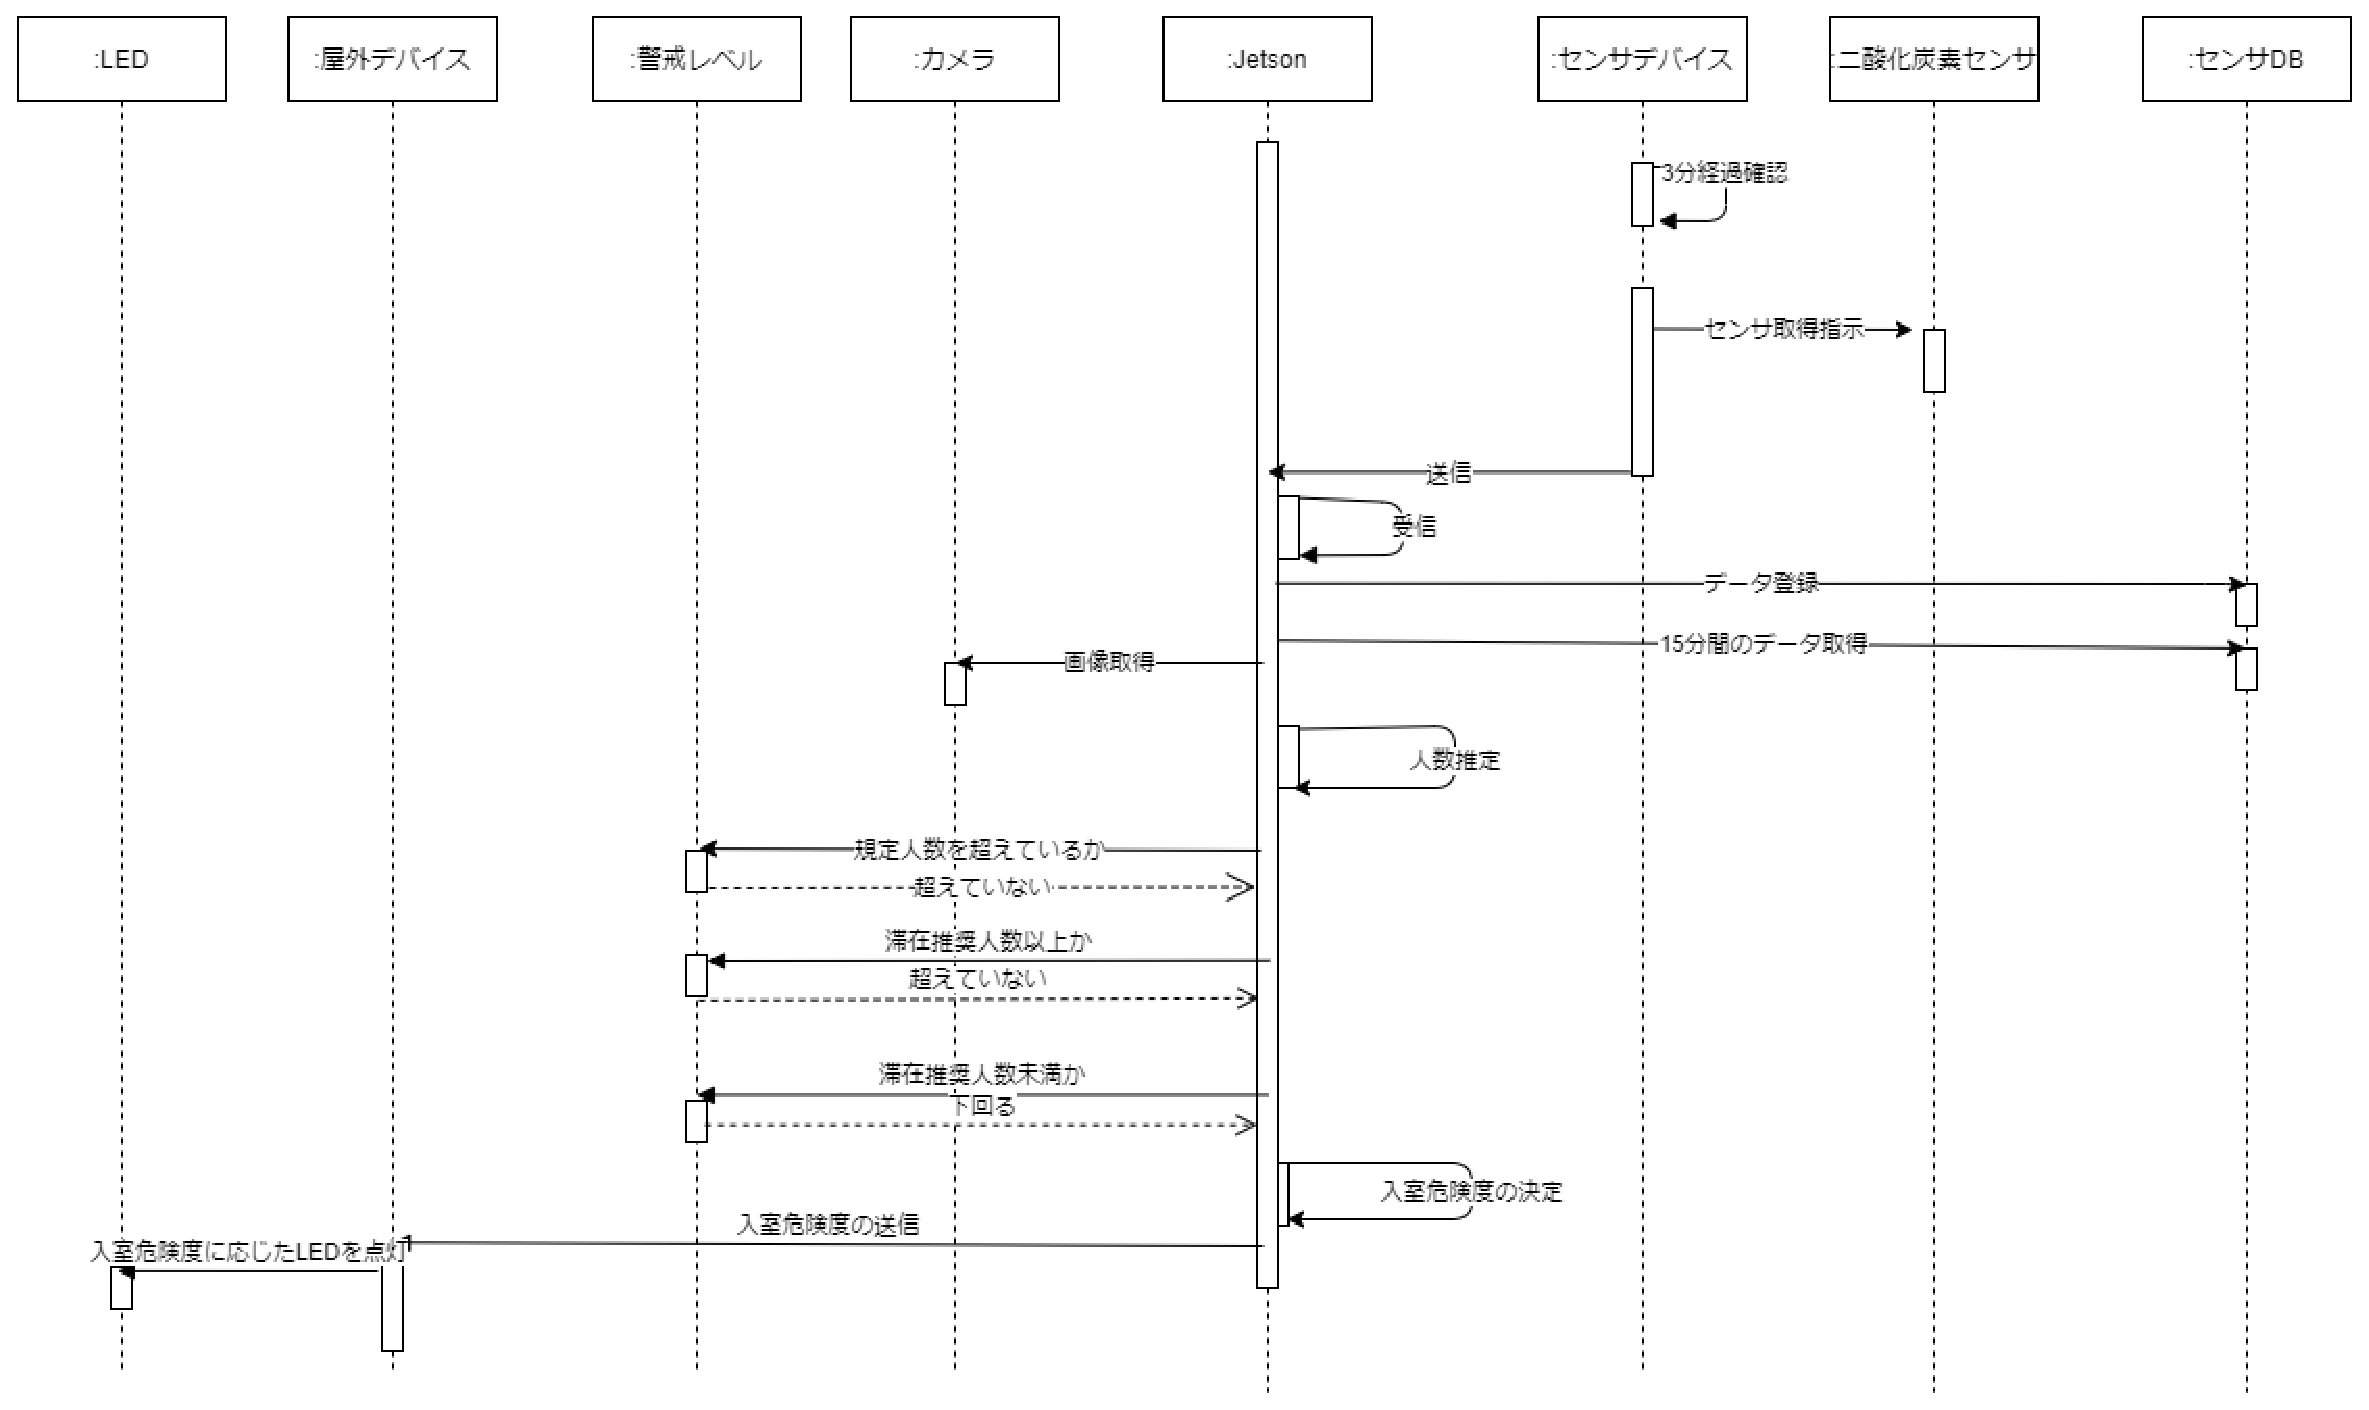
\includegraphics[width = 15cm]{./picture/sequence_nyushitsu_2.eps}
    \caption{ユースケース「入室危険度の確認」のシーケンス図}
    \label{seq_enterlisk}
\end{figure}
\begin{figure}[htbp]
    \centering
    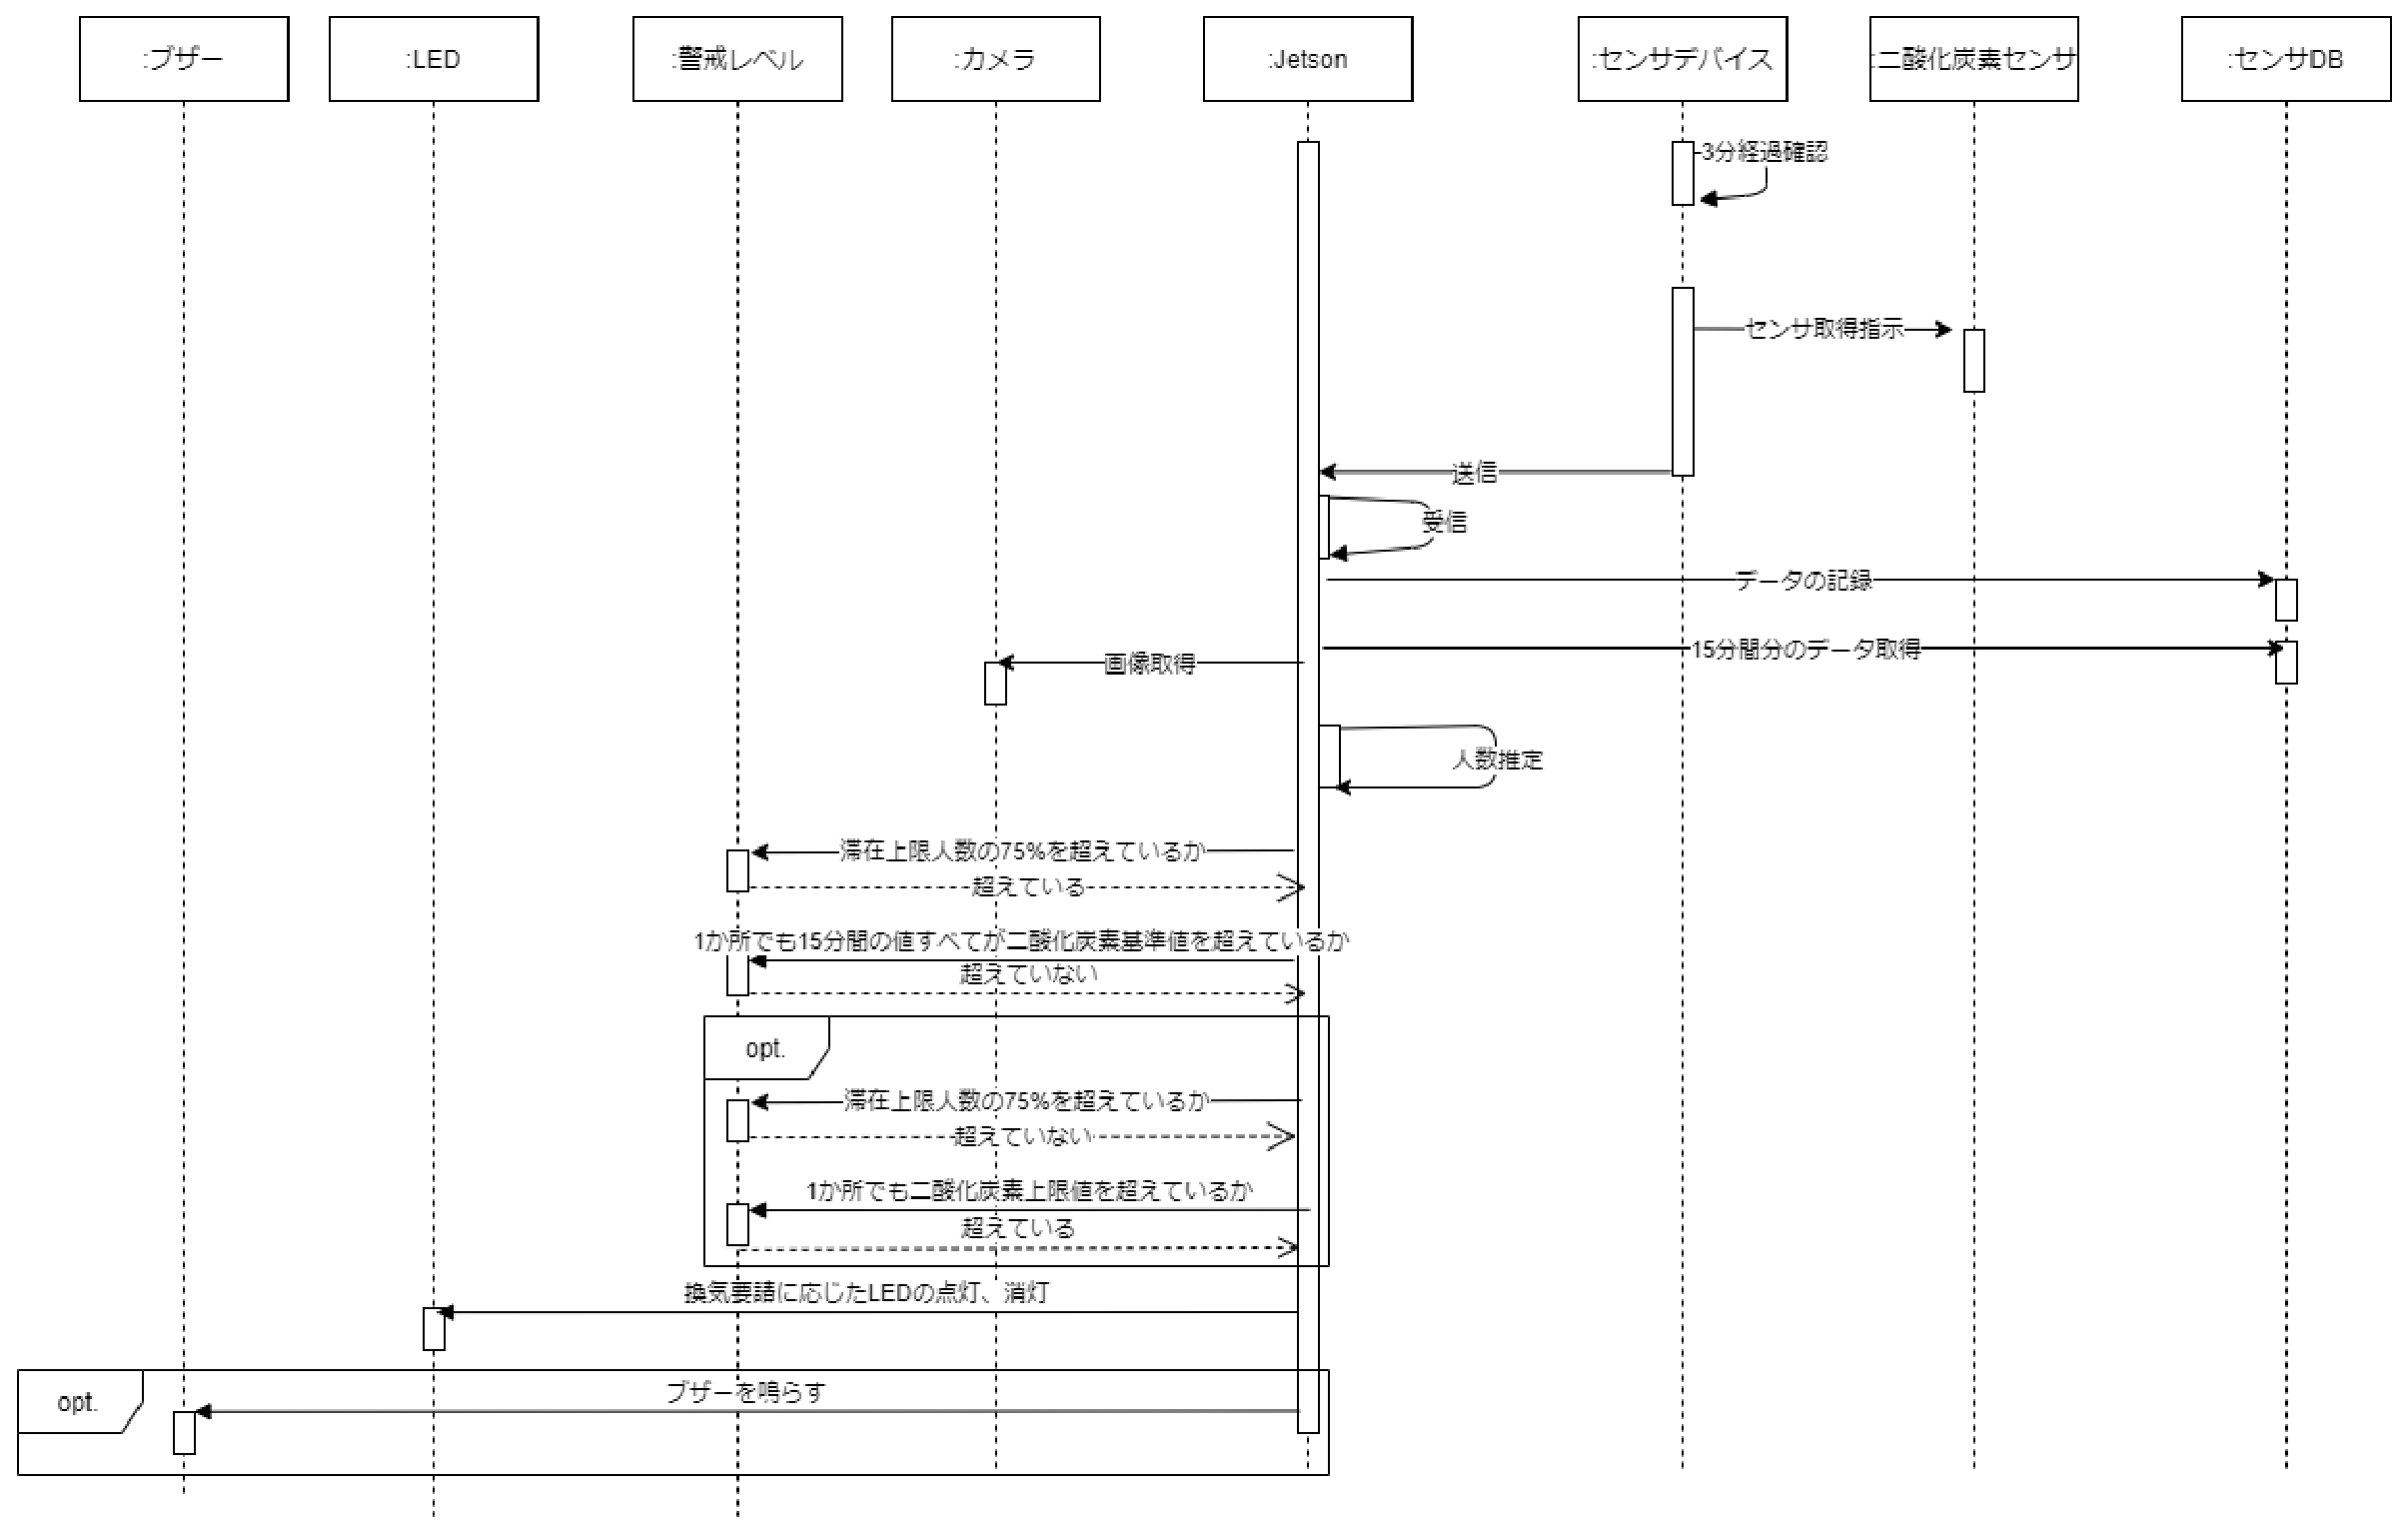
\includegraphics[width = 15cm]{./picture/sequence_kanki_2.eps}
    \caption{ユースケース「換気要請の受け取り」のシーケンス図}
    \label{seq_kanki}
\end{figure}
\begin{figure}[htbp]
    \centering
    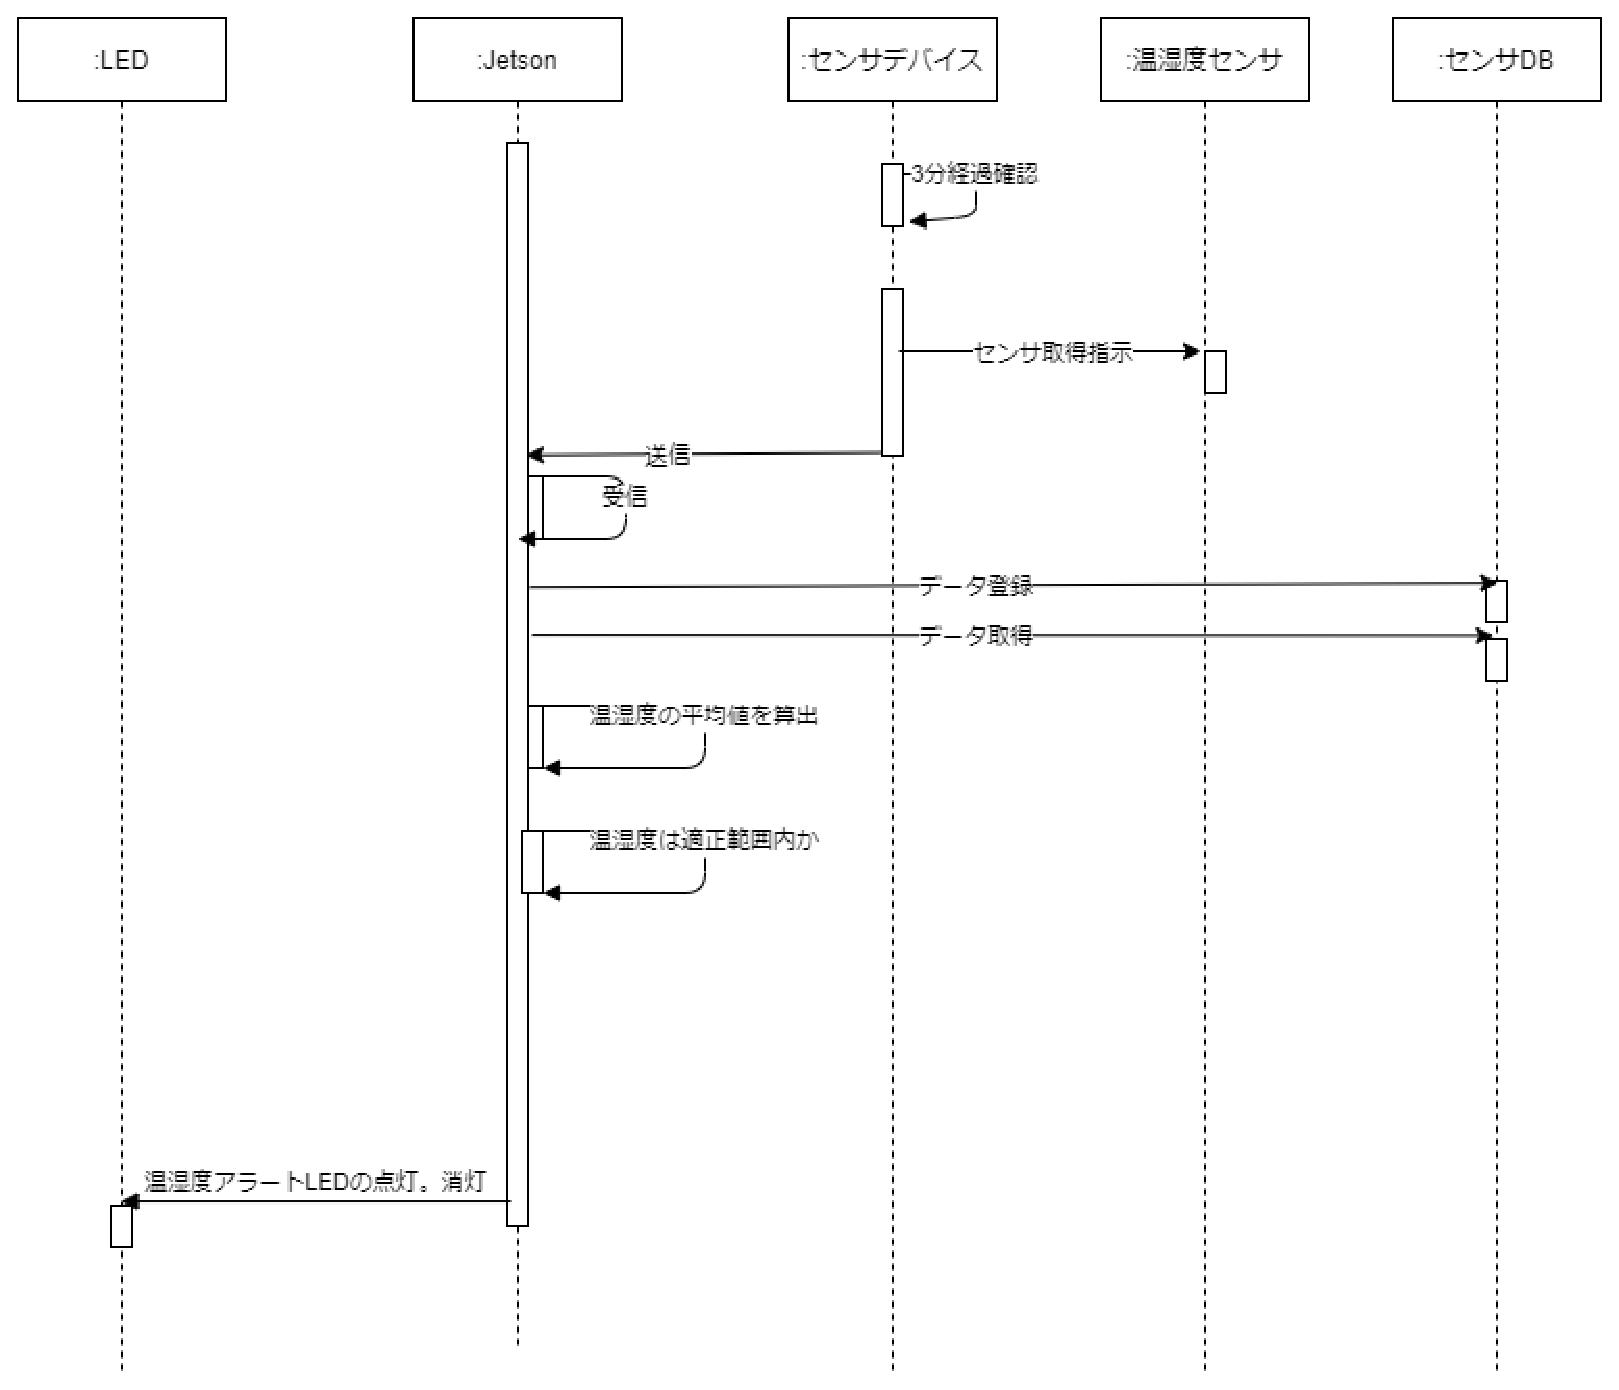
\includegraphics[width = 15cm]{./picture/sequence_shitsunai_2.eps}
    \caption{ユースケース「室内環境状態の表示」のシーケンス図}
    \label{seq_kankyou}
\end{figure}

まず,「室内状況を監視する」際の動作を説明する.
まず,システムが起動され,監視が開始した時には,Jetsonがセンサデバイスに対して開始指示を発する.
それを受け,センサデバイスはセンサからの値取得を行い,Jetsonに送信する.
また,システムが開始された時以外にも,センサデバイスが直近の値取得から3分経過を確認した場合であっても,センサの値取得を行う.
なお,この際送信されるデータは二酸化炭素濃度,温湿度,およびセンサデバイスの識別子である.
Jetsonで受信したデータは,センサDBに登録する.
その後,JetsonはセンサDBより直近15分間分のデータを取り出し,人数推定,および警戒レベルの調整を行う.
受信については,Jetson上で他の処理とは独立したスレッドで行い,受信漏れが起こらないようにする.
スレッド間でのデータのやり取り,および15分間分過去にさかのぼったデータ取得を容易にするため,データの保管にはセンサDBを使用した.
なお,基準値との比較方法について,基準値を上回っているかどうかは,複数あるセンサデバイスのうち一台でも連続して上回っているものがあれば超えているとみなす.
一方,基準値を下回っているかどうかは,複数あるセンサデバイスのすべてが連続して基準値を下回っているかどうかによって判断する.
なお,図\ref{seq_kanshi}では,例として警戒レベルを下げる際の処理の流れを示している.
ほかの場合の処理については,図\ref{act_kanshi}で示した条件に従い,同様に処理が行われる.
また,あらかじめ指定された時間になると監視を一時停止し,再度システムを起動する.
これは消費電力を抑えるために,夜間などの部屋があまり利用されない時間はシステムを停止させるものである.
一時停止したのち,復帰時間になると,再度監視を開始し,センサデバイスへの開始指示から行うこととした.

続いて,「入室危険度の確認」を行う際の動作を説明する.
センサの値を取得し,人数推定を行うまでは上記「室内状況を監視する」場合と同じである.
その後,警戒レベルが保有している規定人数,および滞在推奨人数との比較を行い,その結果をもとにJetsonが入室危険度の判定を行う.
入室危険度は,そのまま屋外デバイスに通知され,屋外デバイスはそれを受けてLEDを点灯させる.
なお,図\ref{seq_enterlisk}では,一例として入室危険度が「青」と判断される場合の動作を示している.
ほかの場合の処理については,図\ref{act_enterlisk}で示した条件に従い,同様に処理が行われる.

次に,「換気要請の受け取り」を行う際の動作を説明する.
センサの値を取得し,人数推定を行うまでは上記「室内状況を監視する」場合と同じである.
その後,警戒レベルが保有している二酸化炭素濃度の基準値と定められている滞在上限人数とをもとに比較し,換気要請の判断を行う.
二酸化炭素濃度の基準値が超えているかどうかは複数あるセンサデバイスのうち,一台でも連続して値が超えているものが存在すれば超えているものとして判断をする.
その後,LEDを光らせる際には,Jetsonから直接接続したLEDの点灯を行い,点灯する場合は同時にブザーも鳴らす.
なお,図\ref{seq_kanki}では,換気要請を行う場合と換気要請を行わない場合の一例の流れを示している.
他の場合の処理については,図\ref{act_kanki}で示した条件に従い,同様に処理が行われる.

最後に,「室内環境状態の表示」を行う際の動作を説明する.
センサの値を取得するまでの動作は上記「室内状況を監視する」場合と同じである.
その後,センサDBより,その時に取得された全センサデバイスの温湿度の値を読み出し,温度,湿度の平均値を求め,それを代表値とする.
その代表値が適正範囲内にあるかどうかを判断し,範囲外であった場合は,Jetsonに接続されているLEDを点灯する.
温湿度が範囲内であった場合にはLEDを消灯させる.
%なお,本システム湿度30\%以上を適正範囲として制定し,温度については定めないこととした.

続いて,私が担当したセンサデバイスの状態遷移について,ステートチャート図を用いて説明する.
センサデバイスのステートチャート図を図\ref{state_sensor}に示す.
\begin{figure}[htbp]
    \centering
    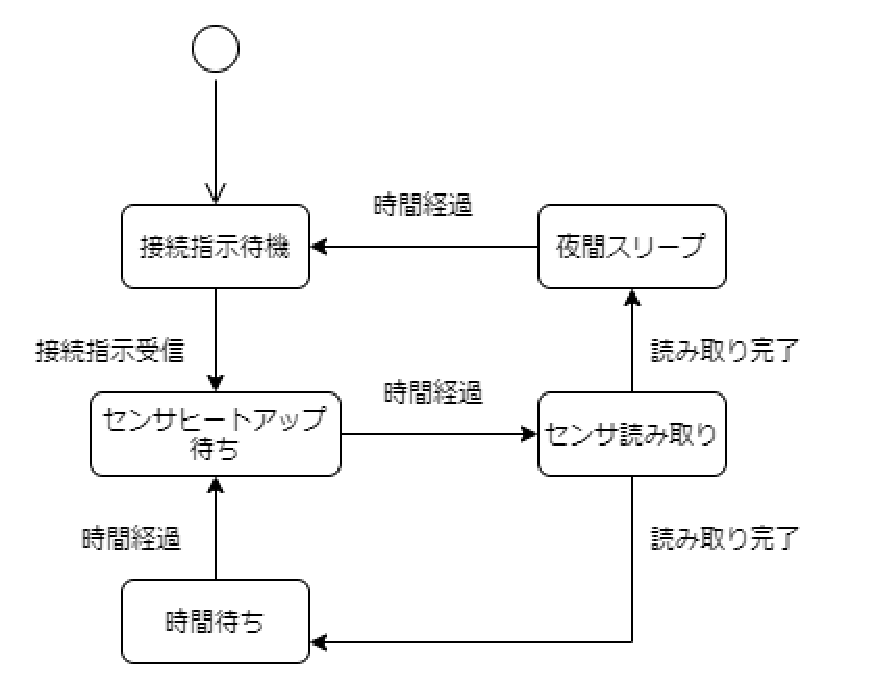
\includegraphics[width = 9cm]{./picture/statechart_micon.eps}
    \caption{センサデバイスのステートチャート図}
    \label{state_sensor}
\end{figure}
センサデバイスの状態は「接続指示待機」,「センサヒートアップ待ち」,「時間待ち」,「夜間スリープ」,「センサ読み取り」の5状態を持つとした.
まず,センサデバイスの電源を入れることで,初期状態の「接続指示待機」状態となる.
この状態では,システムを開始した際,開始指示を受信するまで待機するものである.
その後,「センサヒートアップ待ち」状態へと推移する.
これは,本システムで使用する二酸化炭素濃度センサが,通電直後の場合,正しい値を示さない可能性があり,ヒートアップ時間を必要とするため,その時間を確保するものである.
この間は,マイコンボード,および昇圧センサを介して二酸化炭素濃度センサに電力供給を行う.
なお,この際,センサデバイスが起動している,および受信待機状態であることを確認できるようにするため,この状態のときにはセンサデバイスに接続したLEDを点滅させるようにした.
その後,ヒートアップ時間が経過すると温湿度,二酸化炭素センサの読み取りとJetsonへの送信を行う「センサ読み取り」状態に推移する.
センサの読み取りと送信が終了すると「時間待ち」状態に推移する.
「時間待ち」状態は,二酸化炭素センサへの給電は行わず,できるだけ消費電力を抑えた状態である.
3分毎に値を読み取るので,3分から二酸化炭素センサのヒートアップに要する時間を引いた時間だけこの状態を保つ.
その後,「センサヒートアップ待ち」状態へと戻り,繰り返される.
最後に,あらかじめ指定された時間になると「センサ読み取り」状態からセンサ読み取り,Jetsonへの送信を行ったのち,「夜間スリープ」状態へと推移する.
これは,動作としては「時間待ち」状態と同じく,省電力状態で待つものであるが,これは部屋の利用が少ない時間に推移する状態である.
従って,「時間待ち」状態よりも長い間,この状態を保つことになる.
その後は,マイコンボード内とJetson内のタイマーがずれてしまうことが考えられるため,「接続指示待機」状態へと推移する.
夜間スリープ状態から推移するのは1日に一度であるので,その際に再度接続指示を受け,Jetsonとセンサデバイスの開始時間を1日ごとに同期する狙いがある.
また,「接続指示待機」以外の状態においては,電池の交換時期が分かるよう,供給電力が低くなった際に,センサデバイスに接続したLEDを点灯させることとした.

これらの設計を受け,表\ref{twelite_test_koumoku}の通り,センサデバイスにおける単体テストの項目をデバイスごとに制定した.
\begin{table}[htbp]
    \centering
    \caption{センサデバイスにおける単体テスト項目}
    \label{twelite_test_koumoku}
    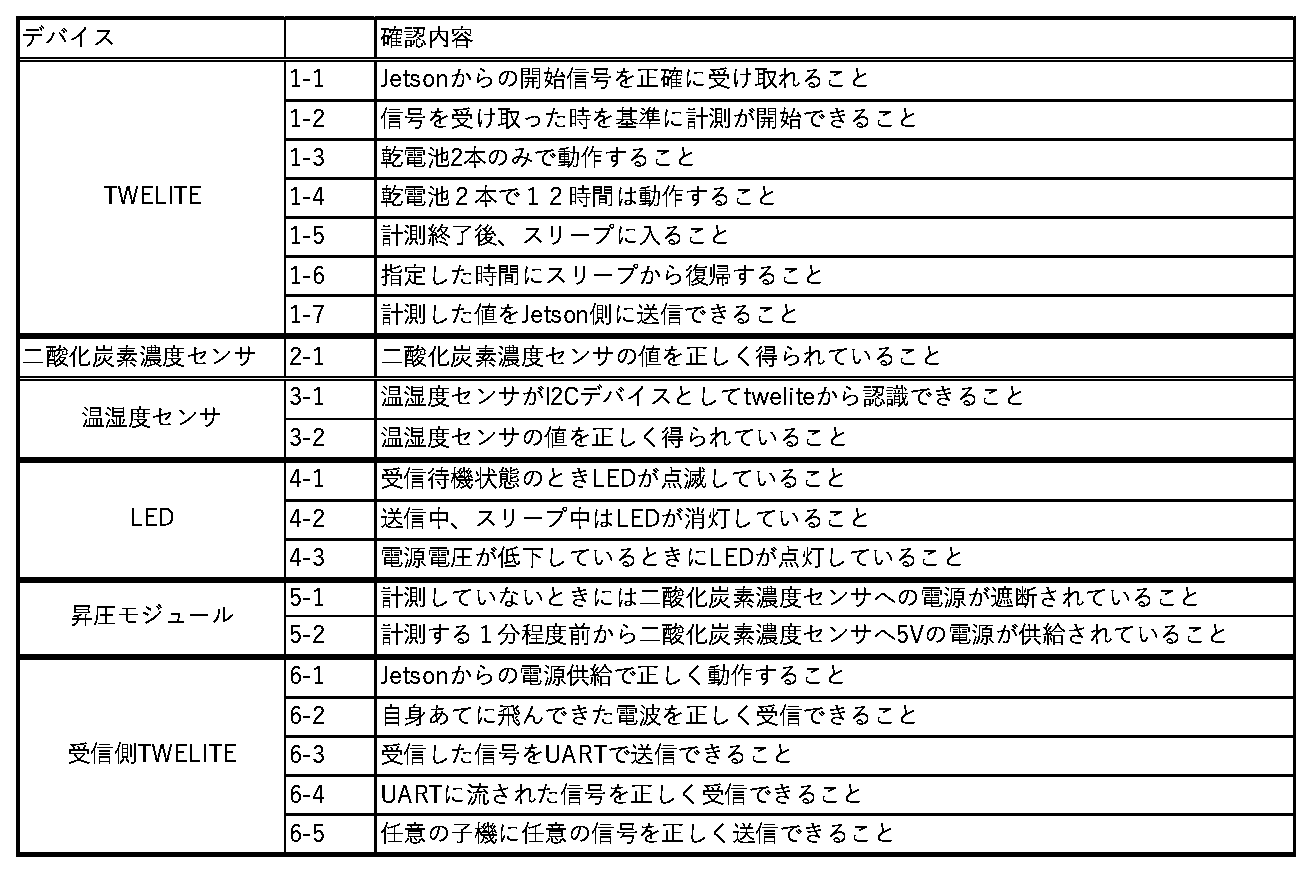
\includegraphics[width = 15cm]{./picture/tantaitest_twelite_koumoku.eps}
\end{table}
なお,消費電力化の目安として,部屋の使用時間が12時間とした際,起動してから最初の「夜間スリープ」状態への遷移が行われるまでは乾電池交換を行うことなく動作できることが最低限必要であるとした.


% オブジェクト間のメッセージのやりとりを時系列に沿って表現するために,シーケンス図を作成した.図\ref{sequence_ic}に,ICタグを用いた商品識別システムのシーケンス図を示す.

% \begin{figure}[htbp]
% \centering
% \includegraphics[width=15cm]{./picture/sequence_ic.eps}
% \caption{ICタグを用いたシステムのシーケンス図}
% \label{sequence_ic}
% \end{figure}


% 図\ref{sequence_qr}はQRコードを用いたシステムのシーケンス図である.


% \begin{figure}[htbp]
% \centering
% \includegraphics[width=15cm]{./picture/sequence_qr.eps}
% \caption{QRコードを用いたシステムのシーケンス図}
% \label{sequence_qr}
% \end{figure}


% 図\ref{sequence_ic}と図\ref{sequence_qr}の違いはユーザ情報の登録の部分のみである.詳細設計まで行ったが,ICタグを用いたシステムとQRコードを用いたシステムの評価は3.2節から大きく変化しなかった.買い物と決済の設計においては共通しているため,そのまま優先度の高いシステムである下記の図\ref{sequence}部分を実装する.



% \begin{figure}[htbp]
% \centering
% \includegraphics[width=15cm]{./picture/sequence.eps}
% \caption{高優先度のシステムのシーケンス図}
% \label{sequence}
% \end{figure}


% 図\ref{sequence}において筆者の担当した部分はメッセージ2~6,10,11の部分である.各メッセージの詳細を下記に示す.


% \begin{quote}
% 2. 超音波センサ反応時にフラグをたてる.

% 3. フラグがたったら,0.5秒に一度,合計6枚の画像を撮り,データ送信用配列にデータを追加する.

% 4. 画像を撮ったことをユーザに知らせるためにLED緑を点灯させる.

% 5. ロードセルより重量が増加したか減少したかを確認し,増加の場合は追加として1,減少の場合は削除として2のフラグをたて,キューへフラグを追加する.ただし,±3gの増減は誤差とする.

% 6. 追加,削除のフラグが入っているキューを参照し,データ送信用配列にフラグ情報を追加し,画像データと合わせてサーバへ送信する.

% 10. バーコード情報を正しく読み取れたか,読み取れなかったかを知らせるフラグをサーバから受信する.

% 11. サーバがバーコード情報を正しく読み取ることができた場合はLED青を,正しく読み取ることができなかった場合はユーザに再度商品の追加,削除を促すためLED赤を点灯させる.
% \end{quote}

% なお,優先度の高い項目部分において,単体テストの際に用いる各センサのテスト項目を下記の表\ref{webcamera},表\ref{chouonpa},表\ref{rodoseru},表\ref{data}に示す.

% \begin{table}[htbp]
% \centering
% \caption{Webカメラの単体テスト項目}
% \includegraphics[width = 15cm]{./picture/webcamera.eps}
% \label{webcamera}
% \end{table}

% \begin{table}[htbp]
% \centering
% \caption{超音波センサの単体テスト項目}
% \includegraphics[width = 15cm]{./picture/chouonpa.eps}
% \label{chouonpa}
% \end{table}

% \begin{table}[htbp]
% \centering
% \caption{ロードセルの単体テスト項目}
% \includegraphics[width = 15cm]{./picture/rodoseru.eps}
% \label{rodoseru}
% \end{table}

% \begin{table}[htbp]
% \centering
% \caption{データ送信の単体テスト項目}
% \includegraphics[width = 15cm]{./picture/data.eps}
% \label{data}
% \end{table}.


%メッセージの説明

%第4章
\chapter{実装・検証}
%第4章:実装・検証

本章ではV字開発モデルの開発プロセスに従い,実装および検証を行った結果を述べる.
4.1節では,各設計に基づいて行った実装について述べる.
4.2節ではそれぞれ詳細設計を単体テスト,基本設計を結合テスト,要求分析を総合テストによって検証した結果を示す.
%第4-1章:実装
%手順(実験者のしたこと)


\section{実装}

本節では設計したものをもとに,実装した環境等について述べる.
本節では私が実装を行った,センサデバイスについてを中心に述べる.

センサデバイスの実装において使用したセンサ,およびモジュールを表\ref{buhin}に示す.
\begin{table}[htb]
\begin{center}
\caption{センサデバイスの実装環境}
\begin{tabular}{|c|c|c|} \hline
種類 & 品名 & 個数 \\ \hline \hline
無線機能付きマイコンボード & TWELITE DIP & 3 \\
温湿度センサ & BME280 & 2 \\
5.0V出力昇圧DCDCコンバータ & AE-XCL102D503CR-G & 2 \\
二酸化炭素濃度センサ & MH-Z14A & 2 \\
LED & OSG8HA3Z74A & 2\\ \hline
\end{tabular}
\label{buhin}
\end{center}
\end{table}
本システムにおいて,センサデバイスは複数用いる想定となっているため,センサデバイスは2つ実装することとした.
また,Jetsonでセンサデバイスへの送受信を行うモジュールも同時に実装を行った.
表\ref{buhin}の個数においては,センサデバイスが2つに加え,Jetsonで用いるモジュールも実装した際の合計個数を示している.

これらの部品を使用し,図\ref{kairozu}のように結線を行い,センサデバイスを実装した.
\begin{figure}[htbp]
    \centering
    \includegraphics[width = 15cm]{./picture/kairozu.eps}
    \caption{センサデバイスの回路図}
    \label{kairozu}
\end{figure}

なお,マイコンボード上で動作するソフトウェアにおいては,TWELITE MWXライブラリを利用し,C++言語を用いて開発を行った.
3章で述べた設計に従い開発を行った.

なお,Jetsonで送受信を行うモジュールについては,UART接続を用い,その信号のやり取りによって送受信を行うこととした.
送信の際には,ネットワーク上の送信先の論理IDとデータをUART通信で受け取り,その内容を即時送信することとした.
受信においては,受信データを確認し,送り元の論理IDとマイコンボードごとに異なるシリアルID,受信電波強度と合わせてUARTへと即時出力することとした.


\subsection*{消費電流の見積り}
表\ref{buhin}のそれぞれ部品のカタログにある平均消費電流値をもとに各状態における消費電流値の概算を行った結果を表\ref{w_risou}に示す.
電圧はすべて3.0Vとして計算しており,有効数字2桁として示している.
なお,「時間待ち」,「夜間スリープ」,「センサヒートアップ待ち」状態においてはマイコンボードはマイコンボードのスリープ機能を用いるものとし,スリープ時の消費電流値を用いた.
\begin{table}[htb]
    \begin{center}
    \caption{消費電流の概算値}
    \begin{tabular}{|c|c|} \hline
状態 &  合計消費電流(mA) \\ \hline \hline
接続指示待機 & 140 \\
センサヒートアップ待ち & 130 \\
センサ読み取り & 140 \\
時間待ち & 0.0051\\
夜間スリープ & 0.0051 \\ \hline
    \end{tabular}
    \label{w_risou}
    \end{center}
\end{table}

表\ref{w_risou}で示した計算の結果をもとに,状態遷移を行う時間間隔等を決定した.
表\ref{w_risou}の結果より,「接続指示待機」,「センサヒートアップ待ち」および「センサ読み取り」状態の消費電力が他と比べて多くなることが予想される.
このことより,これらの状態を保つ時間はできるだけ短くするように調整を行った.
「接続指示待機」,「センサ読み取り」状態からの遷移は時間を設定するものではなく,外部からの信号受信や読み取りが完了することによって行われるため,調整は難しい.
そこで,「センサヒートアップ待ち」状態から「センサ読み取り」状態へと推移する際までの時間を調整することにより省電力化を図った.

まず,二酸化炭素濃度センサが安定して正しい値を示すのにどの程度の時間を要するかを調査した.
二酸化炭素濃度センサに電源供給を行ってから,時間経過に合わせてどのような値が観測されるかを調査した.
方法として,二酸化炭素濃度センサに電源を供給し始めたときから,TWELITEで観測されたアナログ電圧の値を5秒おきに測定することによって調査を行った.
調査に当たっては,MH-Z14Aの説明書に記載されていた「Preheat time」である180秒を参考に,通電開始から210秒間測定を行い,それを数回繰り返した.
観測されたアナログ電圧をもとに,二酸化炭素濃度を算出した結果を図\ref{graph_co2_wait}に示す.
\begin{figure}[htbp]
    \centering
    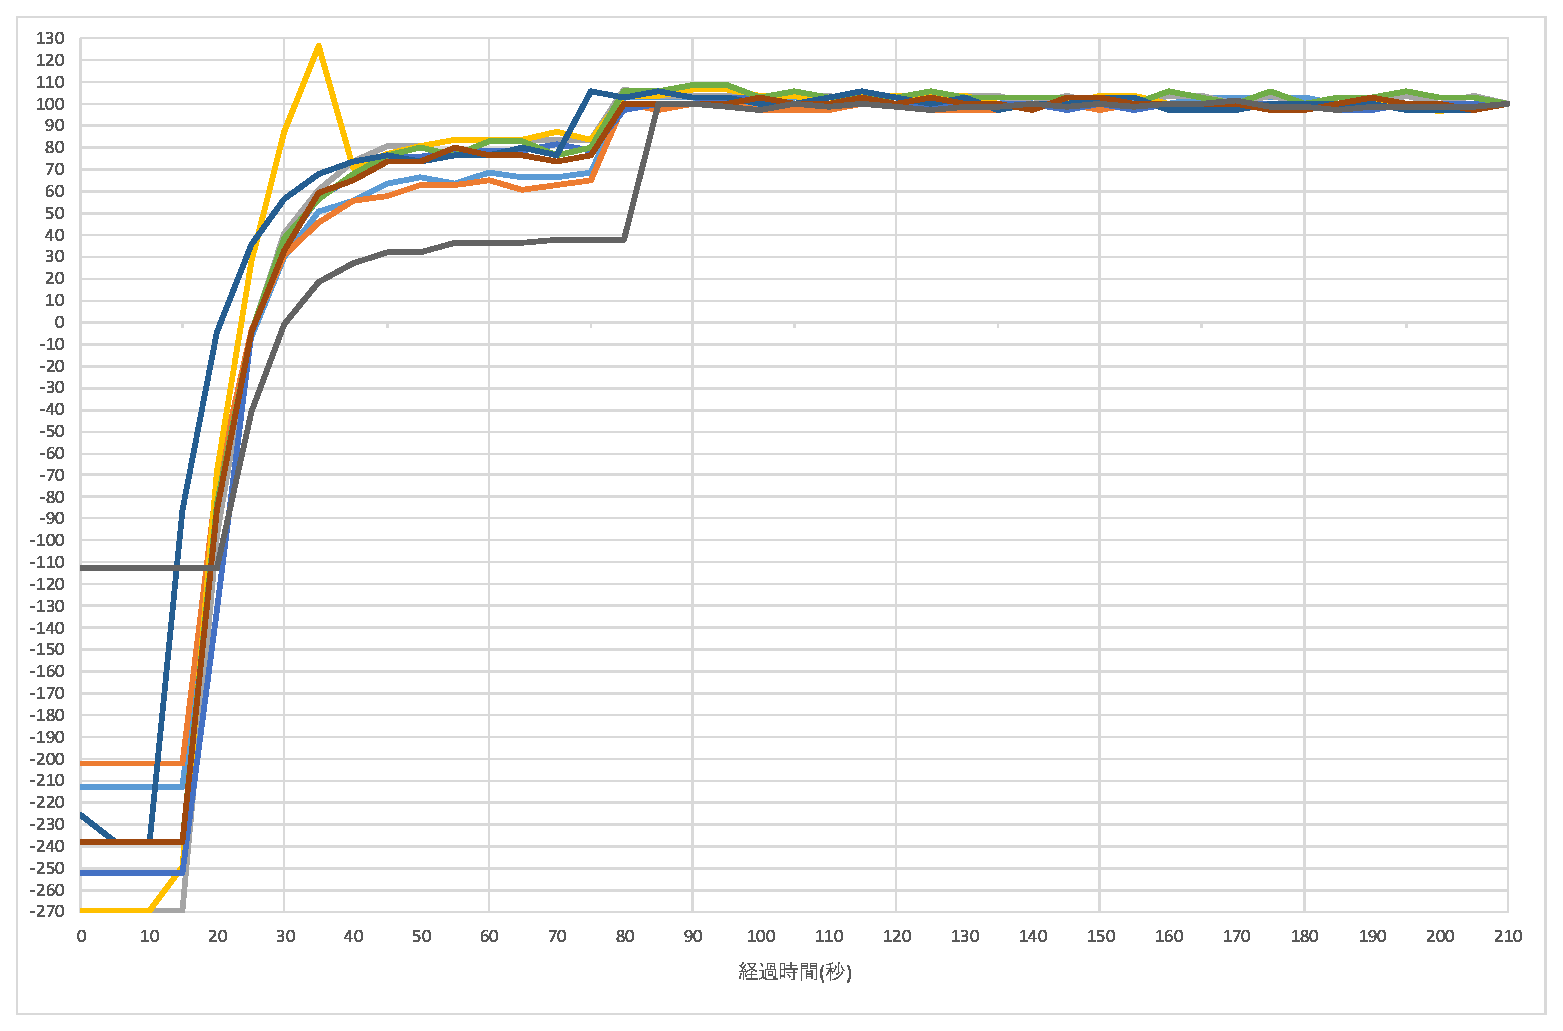
\includegraphics[width = 15cm]{./picture/co2_wait_graph.eps}
    \caption{二酸化炭素濃度センサの観測値の推移}
    \label{graph_co2_wait}
\end{figure}
%図\ref{graph_co2_wait}は横軸に通電開始からの経過時間,縦軸には二酸化炭素濃度0ppmを0として,各回の210秒後に観測された二酸化炭素濃度を100とした時の割合として二酸化炭素濃度を表した数値を示している.
図\ref{graph_co2_wait}は横軸に通電開始からの経過時間,縦軸には観測された二酸化炭素濃度を正規化したものを示している.
二酸化炭素濃度は複数回観測する中で環境を変えると210秒後における最終的な二酸化炭素濃度がそれぞれ異なっていたため,その値がすべて100になるように正規化を行っている.
縦軸で負の値が存在するのは,電圧が0ppmを表す基準電圧よりも低い電圧が観測することがあったため,そのまま二酸化炭素に比例するものとして算出しているためである.
この結果より,通電開始から90秒経過していれば,おおむね正規の値から前後10\%の範囲内の値が観測できることがうかがえる.
そこで,「センサヒートアップ待ち」状態は90秒で次の状態へ遷移するとした.
また,二酸化炭素濃度センサはアナログ電圧の計測時の誤差を少なくするために,10秒ごとに合計3回値の取得を行ったのちに,その平均値を用いて二酸化炭素濃度を推定することとした.
そして,それらをもとに,「時間待ち」状態から「センサヒートアップ待ち」状態へは70秒で推移することとした.

これらの時間の制定を受け,「夜間スリープ」状態を1日12時間制定した場合,1日で消費される推定電池容量の使用量を計算すると,約950mAhとなる.
アルカリ電池単3形を2本用いるとして,1本あたり100mAの連続放電が20時間\cite{denti}であることより,1本あたりの電池容量を2000mAhとすれば,乾電池2本で4日間以上使用可能であると考えられる.
これより,電池交換することなく12時間以上稼働するという設計を満たすことが期待できる.



% 第3章で述べた優先度の高い機能部分について実装を行った.本研究ではグループで開発を行った.サーバ側の精算システムを段原丞治が,Raspberry Piと各種センサを含むモビリティショッピング端末を筆者が実装した.Raspberry Pi はRaspberry Pi 3 Model Bを使用した.Raspberry Piの実装環境については,表\ref{rasp}に示す.


% \begin{table}[htb]
% \begin{center}
% \caption{Raspberry Pi環境}
% \begin{tabular}{|c||c|} \hline
% 使用機器 & Raspberry Pi3 Model B \\ \hline
% OS & raspbian9 \\ \hline
% CPU & 1.2GHz \\ \hline
% メモリ & 1GB \\ \hline
% \end{tabular}
% \label{rasp}
% \end{center}
% \end{table}


% Raspberry Piが制御した各種センサの実装環境について表\ref{jissou}に示す.


% \begin{table}[htb]
% \begin{center}
% \caption{実装環境}
% \begin{tabular}{|c|c|} \hline
% センサ & 個数 \\ \hline \hline
% ロジクール ウェブカメラ C615 & 1 \\
% HY-SRF05超音波距離センサモジュール & 1 \\
% ロードセル シングルポイント(ビーム型)3kg & 1 \\
% SODIAL(R) 100 5mm (LED) & 3 \\ \hline
% \end{tabular}
% \label{jissou}
% \end{center}
% \end{table}


% 上記のセンサをショッピングバスケットに取り付け,実装を行った.表\ref{jissou}に示した各種センサの選定については3.3節に述べたとおりである.ショッピングバスケットのサイズは33L,寸法はW510×D360×H240mmである.ショッピングバスケットを以下カゴと呼ぶ.また,対象の商品として,小規模店舗,中規模店舗にも取り扱いがありそうな菓子としてDARSとコアラのマーチを選定した.

% WebカメラはカゴのW510×D180×H150mmの位置に,カメラを底に向けて設置した.180×180mmのアクリル板をネジでロードセルに留め,Webカメラから100mm下に設置した.超音波センサの設置場所については,Webカメラと同じ高さの2種類の高さの両方の設置場所で実装した.LEDについては緑,青,赤の3色のLEDを抵抗と共にブレッドボードに設置した.カゴに実装したWebカメラ以外の各種センサについては図\ref{sensa}に示す.

% \begin{figure}[htbp]
% \centering
% \includegraphics[width = 15cm]{./picture/sensa_img.eps}
% \caption{各種センサ}
% \label{sensa}
% \end{figure}


% \subsection*{サーバとの通信}

% ユーザが商品を追加,削除した時のみに,Webカメラより画像を撮る.画像データの後に追加もしくは削除のフラグをセットにしてサーバへ送信する.送信のタイミングは3.4節で述べたメッセージにしたがう.

% \subsection*{各種センサの制御}

% それぞれのセンサを制御するためにpythonを開発言語として使用した.センサを稼働し続けるためにはループ処理を行う必要がある.しかしながら,ループ外でセンサが閾値を超えたか否かを確認する必要もあったため,センサの処理は別スレッドで動作させることとした.各センサは以下の動作をさせるよう実装した.

% \noindent
% {\bf ■超音波センサ}

% 商品,もしくは手を感知した際にフラグをたてる.システム起動の際,超音波センサからカゴの端までの距離を測り,その値を初期値とする.その初期値から値が減少していた場合フラグをたてる.ただし,初期値+30mmは誤差とする.

% \noindent
% {\bf ■Webカメラ}

% 超音波センサより,フラグがたった時に0.5秒に一度,合計6枚の画像を撮る.データ送信用配列にデータを追加する.

% \noindent
% {\bf ■ロードセル}

% 重量の増減を感知した際にフラグをたてる.増加したときに1のフラグを,減少した時に2のフラグをたてる.フラグをキューへ追加する.ただし,±3gの増減は誤差とする.

% \noindent
% {\bf ■LED}

% 超音波センサのフラグがたった時,画像撮影開始をユーザに知らせるために緑色のLEDを点灯させる.サーバへデータを送信後,バーコード情報を正しく読み取ることができたというフラグを受けとった際は青色のLEDを,読み取ることができなかったというフラグを受けとった際はユーザに再度商品の追加,削除を促すために赤色のLEDを点灯させる.

% \newpage


%Raspberry Pi側でしたこと
%第4-2章
\section{検証}
ここから、4.1節で実装したプログラムの動作の検証と、他のメンバー担当箇所との統合後の、システム全体の動作の検証を行った。ここでも、V字モデルの開発プロセスに従い、単体テスト、結合テスト、総合テストという順番で検証を行っている。

\subsection{単体テスト}
まずはじめに、実装の段階で検証が求められるレベルの項目について、単体テストを行った。ここでは、実装担当者が中心となって、各担当箇所の検証項目について検証を行った。以下に、私の担当箇所に関する単体テストの内容について述べる。

ここでは、Jetson nano側でのシステム全体の制御に関する部分と、データベース操作に関する部分それぞれについて単体テストを行った。まず、Jetson nano側でのシステム全体の制御に関する部分の単体テストを表\ref{jtantaitest}に示す。

\begin{table}[H]
	\centering
	\caption{jetson nano単体テスト}
	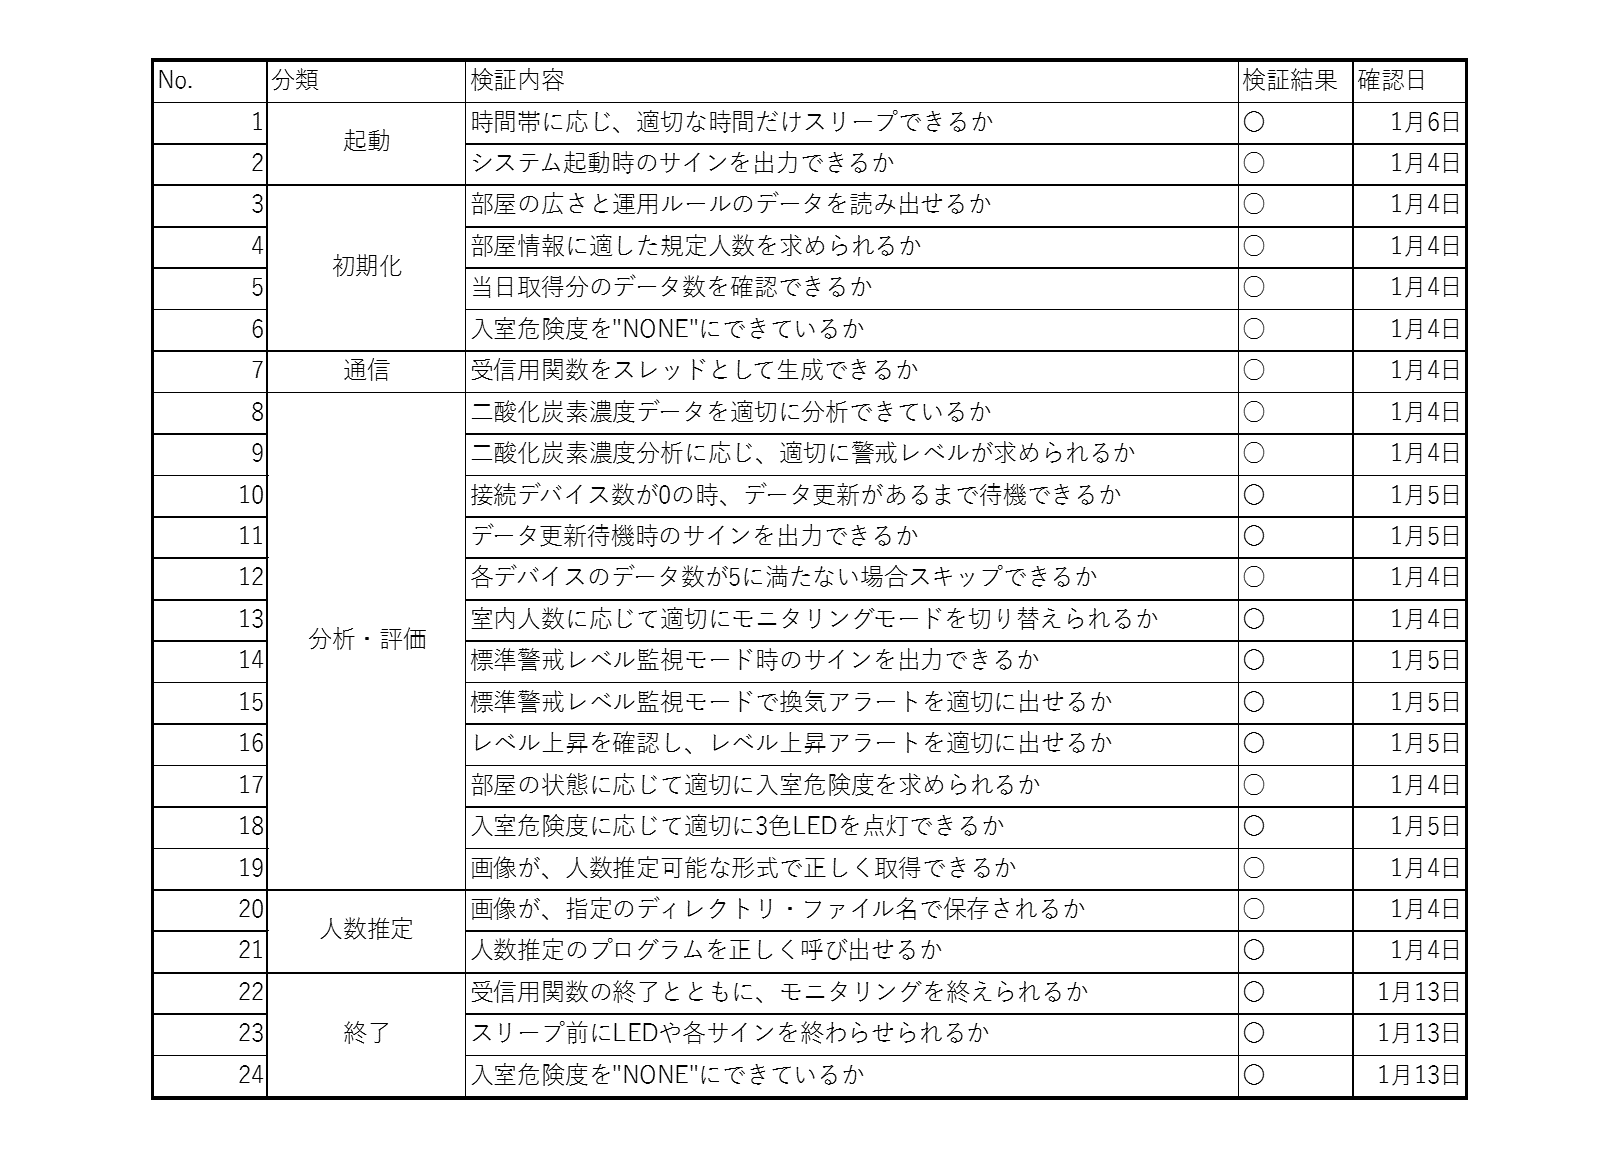
\includegraphics[width=15cm]{jtantaitest.eps}
	\label{jtantaitest}
\end{table}

jetson nano側でデータベース操作以外で実行するのは、4.1節で説明したメインプログラムと各デバイスとの通信用プログラムである。ここではこれらプログラムのうち、メソッドなどの比較的細かな単位で検証を行った。実際のシステム運用時には、他のデバイスとの通信やデータベースの操作などが関わってくるが、手作業で値を与えるなど、疑似的に動作環境をつくり動作を確認した。

ここで特に問題となったのは、LEDを用いた各種サインの出力に関する部分で、それぞれをメインプログラムとは別のスレッドとして生成させて実行するが、状況によっては複数スレッドが同時にGPIOに対し操作してしまう状況があることに気づいた。そのためLEDによるサインを、システム内部の処理によって本来切り替えるべきタイミングで即時切り替えるのではなく、GPIOを操作するスレッドを正常に停止できるまで、GPIOを操作する別スレッドの生成を待機させることでGPIOの操作の一時的な衝突を回避するという修正が必要となった。

続いて、データベース操作に関する部分の単体テストを表\ref{dtantaitest}に示す。

\begin{table}[H]
	\centering
	\caption{データベース単体テスト}
	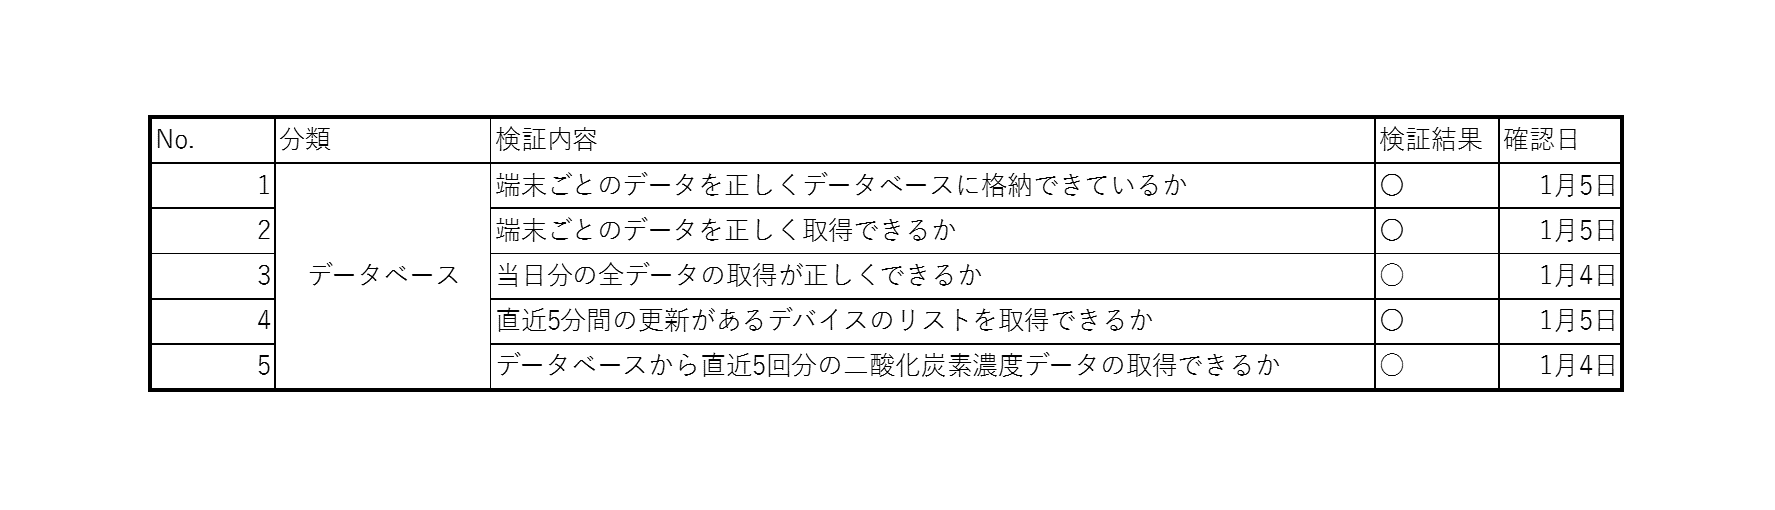
\includegraphics[width=15cm]{dtantaitest.eps}
	\label{dtantaitest}
\end{table}

ここでは、センサデバイスからの取得データに対するデータベースの動作を検証するかわりに、疑似的なデータを与えた場合に、想定した操作を行えるかどうかを検証したが、概ね問題なく動作することが確認できた。

\subsection{結合テスト}
結合テストでは、Jetson nano側で動作するメインプログラムと、データベース操作のプログラムの連携のほか、他のメンバーの担当箇所との統合も含めてテストを行い、デバイス類との通信に関する部分や、人数推定プログラムの動作も検証した。ここで、実施した結合テストを表\ref{ketugoutest}に示す。

\begin{table}[H]
	\centering
	\caption{結合テスト}
	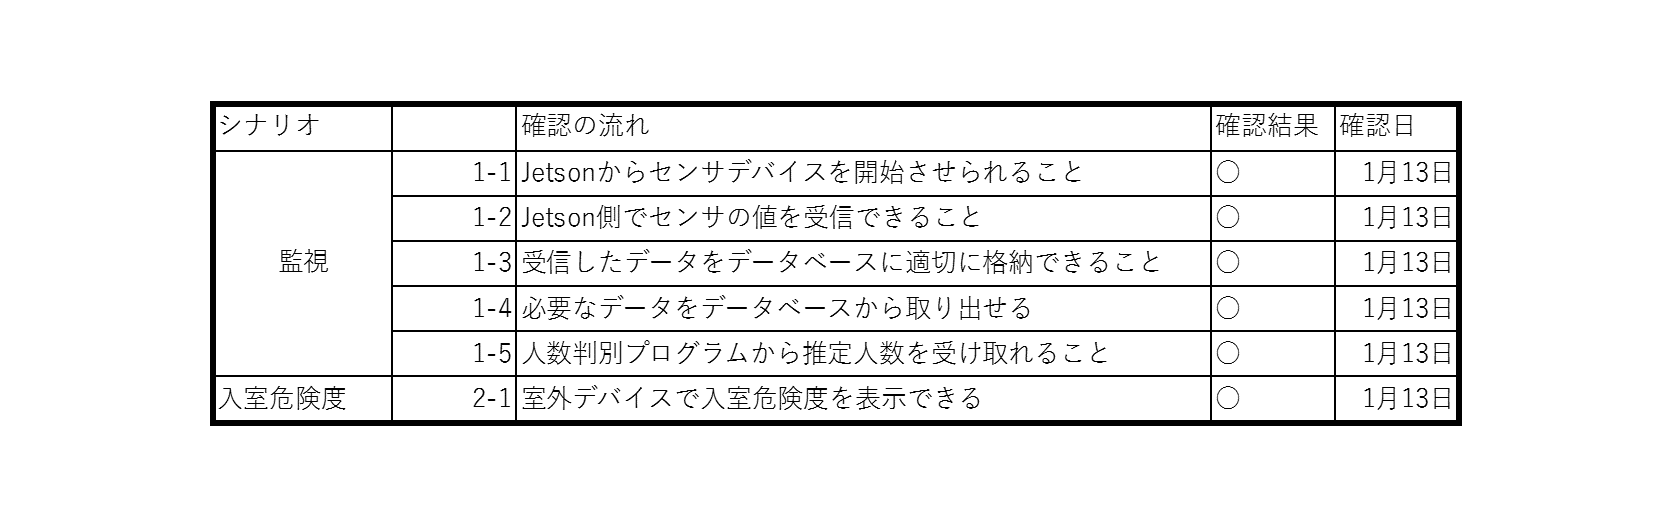
\includegraphics[width=15cm]{ketugoutest.eps}
	\label{ketugoutest}
\end{table}

結合テスト実施までに、各自の担当箇所について単体テストを実施し、プログラムやメソッド、関数等が単体で正常に動作することが確認された。結合テストでは、単体テストの検証項目について、動作が保証されたうえで、それらを組み合わせた場合の動作を確認できた。


\subsection{総合テスト}
総合テストでは、実際の運用を想定した環境で検証を行った。ただし、感染症予防の観点から大人数を集めて、二酸化炭素濃度の変動を確認したり、人数推定プログラムで何十人という人の数をどれくらいの精度で確認できるかといったことまでは、今回は確認することができていない。ここで、実施した総合テストを表\ref{sougoutest}に示す。

\begin{table}[H]
	\centering
	\caption{総合テスト}
	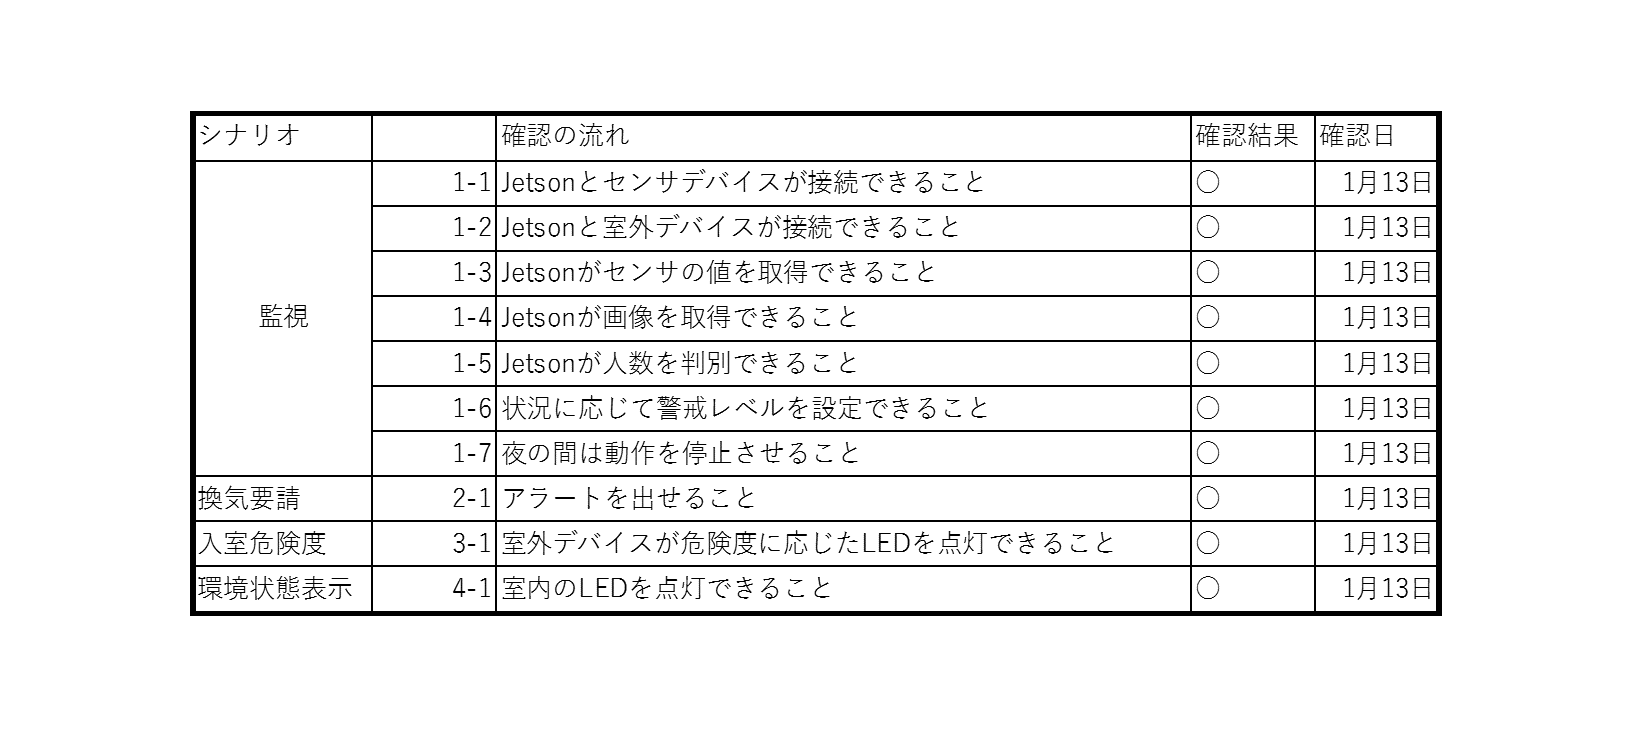
\includegraphics[width=15cm]{sougoutest.eps}
	\label{sougoutest}
\end{table}

このように、最終的に4つのユースケースを満足できることを確認するために、実際のシステム利用環境で検証を行い、各自の担当箇所がうまく統合され、正しく動作することを確認した。

また、デバイス類との接続とデータの取得・管理が正しく動作することを、結合・総合テストの実施によって確認できたことを踏まえ、部屋の滞在人数や換気状況の変化に対するシステムの動作確認を行うために、室内環境を仮想的に表すデータとして、表4.6のようなデータを3分ごとにデータベースに与えて動作させた。なお、表4.6はテストデータを記録したデータベースの内容を示しており、recordIDはレコードに割り当てられた通し番号、dtはセンサデータ取得日時、devIDはセンサデータを送ったデバイスのID、co2が二酸化炭素濃度を示す。以下のデータは、センサデバイス2台の3分おき20回分のデータ取得を想定している。ただし実際には、このほかにもいくつかのフィールドがデータベースに記録されているが、ここでは省略している。


\begin{longtable}{|c|c|c|c|}
	\caption{テストデータ}
	\label{testdata}
	\endhead
	\hline
	recordID & dt & devID & co2\\ \hline \hline
	1 & 2021-01-16 14:38:43 & 1 & 581\\
	2 & 2021-01-16 14:38:43 & 2 & 580\\
	3 & 2021-01-16 14:41:43 & 1 & 587\\
	4 & 2021-01-16 14:41:43 & 2 & 592\\
	5 & 2021-01-16 14:44:43 & 1 & 593\\
	6 & 2021-01-16 14:44:43 & 2 & 603\\ 
	7 & 2021-01-16 14:47:43 & 1 & 622\\ 
	8 & 2021-01-16 14:47:43 & 2 & 621\\ 
	9 & 2021-01-16 14:50:43 & 1 & 644\\ 
	10 & 2021-01-16 14:50:43 & 2 & 656\\ 
	11 & 2021-01-16 14:53:43 & 1 & 667\\ 
	12 & 2021-01-16 14:53:43 & 2 & 694\\
	13 & 2021-01-16 14:56:43 & 1 & 689\\
	14 & 2021-01-16 14:56:43 & 2 & 712\\ 
	15 & 2021-01-16 14:59:43 & 1 & 703\\
	16 & 2021-01-16 14:59:43 & 2 & 739\\
	17 & 2021-01-16 15:02:43 & 1 & 724\\
	18 & 2021-01-16 15:02:43 & 2 & 802\\
	19 & 2021-01-16 15:05:43 & 1 & 769\\
	20 & 2021-01-16 15:05:43 & 2 & 812\\
	21 & 2021-01-16 15:08:43 & 1 & 796\\
	22 & 2021-01-16 15:08:43 & 2 & 833\\
	23 & 2021-01-16 15:11:43 & 1 & 811\\
	24 & 2021-01-16 15:11:43 & 2 & 855\\
	25 & 2021-01-16 15:14:43 & 1 & 824\\
	26 & 2021-01-16 15:14:43 & 2 & 889\\
	27 & 2021-01-16 15:17:43 & 1 & 829\\
	28 & 2021-01-16 15:17:43 & 2 & 856\\
	29 & 2021-01-16 15:20:43 & 1 & 811\\
	30 & 2021-01-16 15:20:43 & 2 & 833\\ 
	31 & 2021-01-16 15:23:43 & 1 & 798\\
	32 & 2021-01-16 15:23:43 & 2 & 791\\
	33 & 2021-01-16 15:26:43 & 1 & 783\\ 
	34 & 2021-01-16 15:26:43 & 2 & 786\\ 
	35 & 2021-01-16 15:29:43 & 1 & 779\\
	36 & 2021-01-16 15:29:43 & 2 & 784\\ 
	37 & 2021-01-16 15:32:43 & 1 & 753\\
	38 & 2021-01-16 15:32:43 & 2 & 779\\
	39 & 2021-01-16 15:35:43 & 1 & 737\\ 
	40 & 2021-01-16 15:35:43 & 2 & 771\\ \hline
\end{longtable}

また、上のデータを与えた場合に求められる、室内の二酸化炭素濃度代表値と警戒レベルは以下のようになり、滞在人数の値に対して、感染リスクが求められる様子を確認した。ただし、システムの運用環境は、広さが100平方メートルで、5平方メートルに1人までが滞在でき、最大で20人までが滞在可能な部屋を想定している。

\begin{longtable}{|c|c|c|c|c|c|}
\caption{分析結果と滞在人数に対するリスク評価}
\label{testresult}
\endhead
\hline
番号 & 日時 & co2代表値 & 警戒レベル & 滞在人数 & 感染リスク\\ \hline \hline
1 & 2021-01-16 14:38:43 & - & 0 & 8 & -\\
2 & 2021-01-16 14:41:43 & - & 0 & 9 & -\\
3 & 2021-01-16 14:44:43 & - & 0 & 8 & -\\
4 & 2021-01-16 14:47:43 & - & 0 & 10 & -\\ 
5 & 2021-01-16 14:50:43 & 581 & 0 & 14 & -\\ 
6 & 2021-01-16 14:53:43 & 592 & 1 & 15 & green\\ 
7 & 2021-01-16 14:56:43 & 603 & 1 & 15 & green\\
8 & 2021-01-16 14:59:43 & 622 & 1 & 17 & green\\
9 & 2021-01-16 15:02:43 & 656 & 1 & 16 & green\\
10 & 2021-01-16 15:05:43 & 694 & 1 & 17 & green\\
11 & 2021-01-16 15:08:43 & 712 & 2 & 17 & green\\
12 & 2021-01-16 15:11:43 & 739 & 2 & 18 & yellow\\
13 & 2021-01-16 15:14:43 & 802 & 3 & 18 & red\\
14 & 2021-01-16 15:17:43 & 812 & 3 & 17 & yellow\\
15 & 2021-01-16 15:20:43 & 833 & 3 & 16 & green\\
16 & 2021-01-16 15:23:43 & 798 & 2 & 15 & green\\
17 & 2021-01-16 15:26:43 & 786 & 2 & 15 & green\\ 
18 & 2021-01-16 15:29:43 & 784 & 2 & 16 & green\\
19 & 2021-01-16 15:32:43 & 779 & 2 & 17 & green\\
20 & 2021-01-16 15:35:43 & 771 & 2 & 18 & yellow\\ \hline
\end{longtable}

以上のデータは、室内にほとんど人がいない状態から徐々に人数が増えていき、二酸化炭素濃度・警戒レベルが上昇し、換気アラートが出され、感染リスクが高まったことを受け、換気が行われ感染リスクが安全水準に戻される様子を想定している。

今回は、初回起動時を想定したため、データの始まりは14時台であるものの二酸化炭素濃度分析のために必要な5回分の取得データがない状態から始まり、警戒レベルは初めに0に設定され、初めの4回分のデータ分析では、部屋の二酸化炭素濃度の代表値は導出されない。このように、データ数が少ない時には、提供できる情報がないものの、システムが稼働していることは利用者に知らせる必要があることから、スタンバイ中であることを示すLEDサインを出力する。また、数分前に感染リスク評価を行っていた場合でも、接続デバイスから長時間データ更新がされなかった場合には、その感染リスクの情報の信憑性が下がることから、同じサインを出力させることとなっている。

5回目以降の分析時には、分析に必要なデータ数が揃ったことで、部屋の二酸化炭素濃度の代表値が定められ、警戒レベルと感染リスクの評価が行われる。ただし、5回目の分析では、室内の滞在人数が20人の75\%を下回るため、警戒レベルとリスクの評価は行われない。

以降のデータ分析に関しても、上で示したテストデータと室内人数から、設計通りの分析ができたことが確認でき、二酸化炭素濃度の上昇に伴って、滞在可能な人数が制限され、より少ない人数しか滞在していない場合でも感染リスクが厳しくつけられ、警戒レベル上昇時に出される換気要請とともに、利用者に対して感染予防のためのアクションを促す機能が、設計通り実現されていることが確認できた。

今回は二酸化炭素濃度や室内の人数の変動を、実際の利用環境で再現することを避けたことから、このようなテスト環境で検証を行うこととなった。実際の利用環境でのテスト稼働時にも、授業などで大人数が出入りし、二酸化炭素濃度が上昇し警戒レベルを高めるような、実際の運用時に想定される環境変化こそ再現できていないものの、実際のシステム利用環境であっても、仮想的な室内環境を想定し、疑似的なデータを与えた検証時と同じように、設計通りの動作ができることが確認された。





%第5章
\chapter{評価・考察}
%第5章
本章では、本システムに対する評価・考察を行い、今後の課題や将来性についても述べる。

まず3.1節に挙げた、本システムが果たすべき2つの大きな役割に対して評価する。3.1節において、本システムが果たすべき役割について、「感染症予防対策のルールを守ってもらうよう働きかける役割」、「感染症予防対策の基準を定める役割」の2つを挙げた。感染症予防対策のルールを守ってもらうよう働きかける役割については、室内環境に応じた換気要請の発出や、感染リスクのレベルの通知によって、換気や人数調整といった具体的なアクションを促すことが実現できていると考えられる。感染症予防対策の基準を定める役割については、利用者が感染症予防のためにとるべき、換気と部屋に滞在する人数の調整というアクションについて、感染症予防の観点から、部屋を安全な状態に保つため、具体的にその基準を定めることで、利用者自身が感染症予防のためにとるべきアクションを明確にすることが実現できていると考えられる。

また本システムでは、センサデバイスで取得したデータを随時データベースに記録しているほか、室内の滞在人数や警戒レベル、感染リスクといったデータも、センサデバイスからのデータ更新に伴って導き出されていることから、必要に応じてデータを保管しておくことで、システム外部で様々なデータの相関を調べることもできる。そのため、感染症予防対策の基準を定める役割に関しては、応用の余地があると考えられ、例えば以下のような応用の仕方が考えられる。

本システムでは、分析に活かせる多くのデータを導き出せるが、中でも設計の段階から分析に役立てられるデータとして着目していたのは、警戒レベルと感染リスクのデータである。既に述べたように、室内にある程度の人数が滞在していないと警戒レベルの導出は行われない。そのため警戒レベルの推移のデータは、その部屋が警戒レベルを導出できる条件下で利用されているとき、どの程度二酸化炭素濃度が高まりやすいかを確認でき、運用ルール改定の基準にできる。また、警戒レベルと感染リスクのデータをシステム内部で分析し、本システムでは固定的である、二酸化炭素濃度と警戒レベル、警戒レベルと滞在可能人数の関係を、部屋の警戒レベルと感染リスクの変動の仕方に応じて流動的に変化させると、よりその部屋にあった感染症予防対策を講じることが可能になると考えられる。

感染リスクのデータは、換気状況など、部屋の運用の仕方が適切であるかどうかを示しているため、部屋が感染症予防対策上、危険な状態で使用されていないかを確認できる。そのため学校やオフィス、公共施設などでの利用のケースを想定すると、時間帯ごとの感染症予防対策への取り組みの徹底度合いが、エビデンスとして残されることから、管理者側からの適切な指導が行えるほか、各部屋の責任者となる者が、感染症予防対策に、より注意して取り組むことができると考える。

本システムの設計時の着想では、利用環境ごとに異なる、床面積の広さ・空間の広さ、換気のしやすさや窓の位置と数、換気設備の有無、部屋利用者の活動の仕方などに柔軟に対応し、利用環境に合わせた感染症予防対策の基準を定め、利用者に感染症予防対策のルールを守ってもらうよう働きかけられることが本システムの特徴であった。実際に、本システムは4.2節の総合テストでの検証のように、様々なシナリオにあった感染症予防の働きかけが可能となることが考えられる。しかしながら、本システムでの感染症予防対策の基準の決め方では、換気のしやすさや、部屋の床面積の広さのわりに、ものが多く置かれているなどの理由から実際の空間が狭いというような部屋の特性が、そのまま二酸化炭素濃度の上昇の仕方に反映されることを前提としている部分があり、柔軟性に欠けていると考える。理想的な環境における本システムの実用性は確認されたものの、部屋ごとの特性を加味した感染症予防対策の基準を、実際の利用環境において適切に定めるためには、本システムでの室内環境の分析の仕方よりも複雑に、室内環境を分析する必要があるとも考えられ、部屋の特性自体をシステムの分析機能によって導き出すことができると、現在のシステムと比較し、よりその部屋の特性に適合した感染症予防対策の基準の設定を行うことができるため、更なる研究と改良の余地が大いに残されていると考える。



%第5-1章:評価

\section{評価}

第3章では,感染症予防サポートシステムは,感染症予防の観点から感染リスクのレベルを通知するとともに,感染リスクを軽減する環境づくりをサポートするという目的を基にして,下記の2点の要求事項を満たす必要があるとした.

\begin{itemize}
	\item 室内環境が測定できること.
	\item 設定した感染リスクの基準に従って通知ができること.
\end{itemize}

「室内環境が測定できること」という要求事項に関して,作成したシステムは二酸化炭素濃度,温湿度,室内滞在人数の測定ができるため,要求を満たすことができたといえる.
「設定した感染リスクの基準に従って通知ができること」という要求事項に関しては,警戒レベル,換気要請の基準,入室危険度を設定し,警戒レベルおよび入室危険度はLED,換気要請はブザーによって,ユーザーに感染リスクの情報を,視覚や聴覚で分かりやすく能動的に通知することができた.室外のユーザーには室外デバイスによるLEDでの入室危険度の通知,室内のユーザーにはブザーとLEDによる換気要請や警戒レベルの通知というように,対象とするユーザーによって提供する情報,提供の方法を変えることで,室内外から共に感染リスクを軽減する環境づくりをサポートするシステムとなった。
%第5章:考察

\section{考察}

今回作成した感染リスク通知デバイスは3色のLEDで入室危険度を分かりやすく表示するというものである.
理想的には,センサーとカメラで収集した施設内の環境情報(在室人数,入室できる人数,二酸化炭素濃度水準,換気状態,感染リスク等の情報)を利用者対象別に提供することが望ましいが,ハードや時間の制約のために,室内外への感染リスクに関する基本的な情報提供機能のみの実装となり,すべての環境情報をユーザーに知らせるまで至らなかった.
しかしながら,在室人数,入室可能人数,二酸化炭素濃度等の数値に関して,本システムはデータを収集できている.
今後,ディスプレイ等を使用すれば,Jetsonから各種データを受け取ることで室内外により詳細な環境情報を表示することができると考える.


%第6章
\chapter{あとがき}
%あとがき
本研究ではセンシング技術、物体検出技術、および複数デバイス間の無線通信という3つの技術とデータ分析の組み合わせによって、感染症予防という、研究・実用化が活発に進められる分野において新たな価値を生み出すことができた。感染症予防に関しては、既に様々な分野で研究・開発がなされているものと思われるが、今回私たちが開発したシステムも、感染症予防の取組を援用するシステムとして貢献できると考える。

また今回の研究では、感染症予防のために活用できるシステムの社会的な必要性が高まり、多くの企業や研究機関により研究・開発が進められている状況下で、感染症予防のために用いるシステムとして、3 密回避に役立てられるという、新型コロナウイルスの世界的な流行以前にはなかった新しい価値を持たせることも、1つの目標として定められた。本研究において、私たちの考える感染症予防のサポートシステムの基本形を提案することができた。今後さらなる研究が進められれば、より高いリアルタイム性と精度を併せ持つモニタリングと、感染症予防対策基準の設定機能における更なる柔軟性を実現でき、より利用しやすいものへと改良が進められることから、拡張性のある研究であると考える。

%--ここまで本文--


%謝辞
\newpage
\addcontentsline{toc}{chapter}{\protect\numberline{謝辞}{}}
\chapter*{謝辞}
%--ここから謝辞--
本研究を進めるにあたり,懇篤な御指導,御鞭撻を賜わりました本学高橋寛教授に深く御礼申し上げます.

%本論文の作成に関し,詳細なるご検討,貴重な御教示を頂きました本学樋上喜信准教授ならびに王森レイ講師に深く御礼申し上げます.
本論文の作成に関し,詳細なるご検討,貴重な御教示を頂きました本学甲斐博准教授ならびに王森レイ講師に深く御礼申し上げます.
%--審査員決定後に入力
また,審査頂いた本学高橋寛教授ならびに井門俊講師,稲元勉講師に深く御礼申し上げます.

最後に,多大な御協力と貴重な御助言を頂いた本学工学部情報工学科情報システム工学講座高橋研究室の諸氏に厚く御礼申し上げます.

%--ここまで謝辞--

%参考文献
\begin{thebibliography}{99}
%ここから参考文献

%--例--
\bibitem{ishiki}
オムロン ヘルスケア株式会社,新型コロナウイルス感染症の流行における意識と生活習慣の変化 | ニュースリリース|企業情報|オムロン ヘルスケア,https://www.healthcare.omron.co.jp/corp/news/2020/0515.html,2020-5

\bibitem{koronaQA}
厚生労働省,新型コロナウイルスに関するQ\&A(一般の方向け)|厚生労働省,https://www.mhlw.go.jp/stf/seisakunitsuite/bunya/\\kenkou\_iryou/dengue\_fever\_qa\_00001.html,2020-12-24

\bibitem{kanki}
厚生労働省,「換気の悪い密閉空間」を改善するための換気の方法,https://www.mhlw.go.jp/content/10900000/000618969.pdf,2020-4-3

\bibitem{ieee}
IEEE,IEEE 802.15.4,https://www.ieee802.org/15/pub/TG4.html,2021-1-6

\bibitem{wnet}
塚本和也,無線ネットワークシステムのしくみ -IoTを支える基盤技術-,共立出版株式会社,2017

\bibitem{iot}
渡辺晴美,今村誠,久住憲嗣,つながる!基礎技術 IoT入門 -コンピュータ・ネットワーク・データの基礎から開発まで-,株式会社コロナ社,2020

% \bibitem{population}
% 平成28年版 情報通信白書|人口減少社会の到来,総務省,https://www.soumu.go.jp/johotsusintokei/whitepaper/ja/h28/html/nc111110.html,2016-07


% \bibitem{super}
% 一般社団法人 全国スーパーマーケット協会,年次統計調査 2019年調査,http://www.super.or.jp/wp-content/uploads/2019/10/2019nenji-tokei.pdf,2019-10


%変わりなし
\bibitem{uml}
株式会社 オージス総研,かんたんUML[増補改訂版],株式会社 翔泳社,2003

\bibitem{jetson}
NVIDIA Corporation,NVIDIA Jetson が提供する組込みシステムの開発者キットとモジュール,https://www.nvidia.com/ja-jp/autonomous-machines/embedded-systems/,2021-1-13

\bibitem{twelite}
モノワイヤレス株式会社,モノをつなぐ無線マイコンモジュール TWELITE-トワイライト - MONO-WIRELESS.COM,https://mono-wireless.com/jp/products/TWE-LITE/index.html,2021-1-13

\bibitem{kumikomi}
阪田史郎,高田広章,組込みシステム,株式会社 オーム社,2006

\bibitem{denti}
パナソニック株式会社,\newline [アルカリ・マンガン] 乾電池の電池容量はどれ位? PZ29060 - 乾電池 - Panasonic,https://jpn.faq.panasonic.com/app/answers/detail/a\_id/29060/p/1844,1845,1846/\\related/1,2021-01-15

\bibitem{co2_ave}
気象庁,気象庁 | 二酸化炭素濃度の観測結果,https://ds.data.jma.go.jp/ghg/kanshi/obs/co2\_yearave.html,2020-3-24

\bibitem{amedas}
気象庁,2021年01月27日 松山(マツヤマ) 毎正時の観測データ,http://www.jma.go.jp/jp/amedas\_h/today-73166.html,2021-1-27
% \bibitem{soft}
% 小泉寿男,辻 秀一,吉田 幸二,中島 毅,ソフトウェア開発,株式会社 オーム社,2003


% \bibitem{reji}
% レジチョイス編集部,価格・製品特徴比較,https://rejichoice.jp/semi-self-regi/,2020-01-15

%ここまで参考文献

\end{thebibliography}
\end{document}
